% Options for packages loaded elsewhere
\PassOptionsToPackage{unicode}{hyperref}
\PassOptionsToPackage{hyphens}{url}
%
\documentclass[
  ignorenonframetext,
]{beamer}
\usepackage{pgfpages}
\setbeamertemplate{caption}[numbered]
\setbeamertemplate{caption label separator}{: }
\setbeamercolor{caption name}{fg=normal text.fg}
\beamertemplatenavigationsymbolsempty
% Prevent slide breaks in the middle of a paragraph
\widowpenalties 1 10000
\raggedbottom
\setbeamertemplate{part page}{
  \centering
  \begin{beamercolorbox}[sep=16pt,center]{part title}
    \usebeamerfont{part title}\insertpart\par
  \end{beamercolorbox}
}
\setbeamertemplate{section page}{
  \centering
  \begin{beamercolorbox}[sep=12pt,center]{part title}
    \usebeamerfont{section title}\insertsection\par
  \end{beamercolorbox}
}
\setbeamertemplate{subsection page}{
  \centering
  \begin{beamercolorbox}[sep=8pt,center]{part title}
    \usebeamerfont{subsection title}\insertsubsection\par
  \end{beamercolorbox}
}
\AtBeginPart{
  \frame{\partpage}
}
\AtBeginSection{
  \ifbibliography
  \else
    \frame{\sectionpage}
  \fi
}
\AtBeginSubsection{
  \frame{\subsectionpage}
}
\usepackage{amsmath,amssymb}
\usepackage{lmodern}
\usepackage{ifxetex,ifluatex}
\ifnum 0\ifxetex 1\fi\ifluatex 1\fi=0 % if pdftex
  \usepackage[T1]{fontenc}
  \usepackage[utf8]{inputenc}
  \usepackage{textcomp} % provide euro and other symbols
\else % if luatex or xetex
  \usepackage{unicode-math}
  \defaultfontfeatures{Scale=MatchLowercase}
  \defaultfontfeatures[\rmfamily]{Ligatures=TeX,Scale=1}
\fi
% Use upquote if available, for straight quotes in verbatim environments
\IfFileExists{upquote.sty}{\usepackage{upquote}}{}
\IfFileExists{microtype.sty}{% use microtype if available
  \usepackage[]{microtype}
  \UseMicrotypeSet[protrusion]{basicmath} % disable protrusion for tt fonts
}{}
\makeatletter
\@ifundefined{KOMAClassName}{% if non-KOMA class
  \IfFileExists{parskip.sty}{%
    \usepackage{parskip}
  }{% else
    \setlength{\parindent}{0pt}
    \setlength{\parskip}{6pt plus 2pt minus 1pt}}
}{% if KOMA class
  \KOMAoptions{parskip=half}}
\makeatother
\usepackage{xcolor}
\IfFileExists{xurl.sty}{\usepackage{xurl}}{} % add URL line breaks if available
\IfFileExists{bookmark.sty}{\usepackage{bookmark}}{\usepackage{hyperref}}
\hypersetup{
  pdftitle={An Introduction to R},
  pdfauthor={Reio Tanji; Osaka Univ., Graduate School of Econ.},
  hidelinks,
  pdfcreator={LaTeX via pandoc}}
\urlstyle{same} % disable monospaced font for URLs
\newif\ifbibliography
\usepackage{color}
\usepackage{fancyvrb}
\newcommand{\VerbBar}{|}
\newcommand{\VERB}{\Verb[commandchars=\\\{\}]}
\DefineVerbatimEnvironment{Highlighting}{Verbatim}{commandchars=\\\{\}}
% Add ',fontsize=\small' for more characters per line
\usepackage{framed}
\definecolor{shadecolor}{RGB}{248,248,248}
\newenvironment{Shaded}{\begin{snugshade}}{\end{snugshade}}
\newcommand{\AlertTok}[1]{\textcolor[rgb]{0.94,0.16,0.16}{#1}}
\newcommand{\AnnotationTok}[1]{\textcolor[rgb]{0.56,0.35,0.01}{\textbf{\textit{#1}}}}
\newcommand{\AttributeTok}[1]{\textcolor[rgb]{0.77,0.63,0.00}{#1}}
\newcommand{\BaseNTok}[1]{\textcolor[rgb]{0.00,0.00,0.81}{#1}}
\newcommand{\BuiltInTok}[1]{#1}
\newcommand{\CharTok}[1]{\textcolor[rgb]{0.31,0.60,0.02}{#1}}
\newcommand{\CommentTok}[1]{\textcolor[rgb]{0.56,0.35,0.01}{\textit{#1}}}
\newcommand{\CommentVarTok}[1]{\textcolor[rgb]{0.56,0.35,0.01}{\textbf{\textit{#1}}}}
\newcommand{\ConstantTok}[1]{\textcolor[rgb]{0.00,0.00,0.00}{#1}}
\newcommand{\ControlFlowTok}[1]{\textcolor[rgb]{0.13,0.29,0.53}{\textbf{#1}}}
\newcommand{\DataTypeTok}[1]{\textcolor[rgb]{0.13,0.29,0.53}{#1}}
\newcommand{\DecValTok}[1]{\textcolor[rgb]{0.00,0.00,0.81}{#1}}
\newcommand{\DocumentationTok}[1]{\textcolor[rgb]{0.56,0.35,0.01}{\textbf{\textit{#1}}}}
\newcommand{\ErrorTok}[1]{\textcolor[rgb]{0.64,0.00,0.00}{\textbf{#1}}}
\newcommand{\ExtensionTok}[1]{#1}
\newcommand{\FloatTok}[1]{\textcolor[rgb]{0.00,0.00,0.81}{#1}}
\newcommand{\FunctionTok}[1]{\textcolor[rgb]{0.00,0.00,0.00}{#1}}
\newcommand{\ImportTok}[1]{#1}
\newcommand{\InformationTok}[1]{\textcolor[rgb]{0.56,0.35,0.01}{\textbf{\textit{#1}}}}
\newcommand{\KeywordTok}[1]{\textcolor[rgb]{0.13,0.29,0.53}{\textbf{#1}}}
\newcommand{\NormalTok}[1]{#1}
\newcommand{\OperatorTok}[1]{\textcolor[rgb]{0.81,0.36,0.00}{\textbf{#1}}}
\newcommand{\OtherTok}[1]{\textcolor[rgb]{0.56,0.35,0.01}{#1}}
\newcommand{\PreprocessorTok}[1]{\textcolor[rgb]{0.56,0.35,0.01}{\textit{#1}}}
\newcommand{\RegionMarkerTok}[1]{#1}
\newcommand{\SpecialCharTok}[1]{\textcolor[rgb]{0.00,0.00,0.00}{#1}}
\newcommand{\SpecialStringTok}[1]{\textcolor[rgb]{0.31,0.60,0.02}{#1}}
\newcommand{\StringTok}[1]{\textcolor[rgb]{0.31,0.60,0.02}{#1}}
\newcommand{\VariableTok}[1]{\textcolor[rgb]{0.00,0.00,0.00}{#1}}
\newcommand{\VerbatimStringTok}[1]{\textcolor[rgb]{0.31,0.60,0.02}{#1}}
\newcommand{\WarningTok}[1]{\textcolor[rgb]{0.56,0.35,0.01}{\textbf{\textit{#1}}}}
\usepackage{longtable,booktabs,array}
\usepackage{calc} % for calculating minipage widths
\usepackage{caption}
% Make caption package work with longtable
\makeatletter
\def\fnum@table{\tablename~\thetable}
\makeatother
\setlength{\emergencystretch}{3em} % prevent overfull lines
\providecommand{\tightlist}{%
  \setlength{\itemsep}{0pt}\setlength{\parskip}{0pt}}
\setcounter{secnumdepth}{-\maxdimen} % remove section numbering
\ifluatex
  \usepackage{selnolig}  % disable illegal ligatures
\fi

\title{An Introduction to R}
\author{Reio Tanji \and Osaka Univ., Graduate School of Econ.}
\date{April, 2022}

\begin{document}
\frame{\titlepage}

\begin{frame}{はじめに}
\protect\hypertarget{ux306fux3058ux3081ux306b}{}
\begin{itemize}
\tightlist
\item
  このスライドはhtml形式で保存しています

  \begin{itemize}
  \tightlist
  \item
    左下のハンバーガーアイコンをクリックすると各ページに飛べます
  \item
    ただ、PC以外の方法で閲覧するのはちょっと不便
  \end{itemize}
\item
  ファイルをpdfで保存することができます

  \begin{itemize}
  \tightlist
  \item
    ブラウザURLの末尾の``\textasciitilde html''の後ろに``?print-pdf''を付け、ページを印刷するとpdf形式で保存できます
  \item
    紙に印刷して見たい、単純に見づらいからpdfで閲覧したいという方はどうぞ
  \end{itemize}
\end{itemize}

\begin{block}{関係資料}
\protect\hypertarget{ux95a2ux4fc2ux8cc7ux6599}{}
\begin{itemize}
\tightlist
\item
  このスライドを含めた資料は以下のURLからダウンロードできます

  \begin{itemize}
  \tightlist
  \item
    \href{https://raw.githubusercontent.com/T-Reio/r_introduction/main/script/script_sample.R}{スクリプトのサンプル}
  \item
    名前を付けて保存→ファイルの種類を「すべてのファイル」に変更して、末尾が「.R」で終わる名前にする
  \end{itemize}
\item
  適宜更新していく(予定)ので、たまにチェックしてみて下さい

  \begin{itemize}
  \tightlist
  \item
    スライドは綺麗に上がらなかったので、来週分はまたSlack (山本先生経由)
    でお送りします
  \end{itemize}
\end{itemize}
\end{block}

\begin{block}{自己紹介}
\protect\hypertarget{ux81eaux5df1ux7d39ux4ecb}{}
\begin{itemize}
\tightlist
\item
  丹治 伶峰 (たんじ れいお)

  \begin{itemize}
  \tightlist
  \item
    大阪大学大学院 博士後期課程
  \item
    大阪大学経済学部卒業 (2018)

    \begin{itemize}
    \tightlist
    \item
      学部時代は準硬式野球部に所属してました
    \end{itemize}
  \item
    専門: 労働経済学・行動経済学

    \begin{itemize}
    \tightlist
    \item
      野球のデータを使って色々してます
    \item
      野球以外もしてます
    \end{itemize}
  \item
    趣味: 音楽聴く、Fantasy Baseball
  \end{itemize}
\item
  よろしくおねがいします
\end{itemize}
\end{block}
\end{frame}

\begin{frame}[fragile]{R言語を使う}
\protect\hypertarget{rux8a00ux8a9eux3092ux4f7fux3046}{}
\begin{itemize}
\tightlist
\item
  R言語とは?
\item
  Rでできること

  \begin{itemize}
  \tightlist
  \item
    研究・分析のフロー
  \end{itemize}
\item
  R言語の基本構造
\end{itemize}

\begin{block}{R言語とは?}
\protect\hypertarget{rux8a00ux8a9eux3068ux306f}{}
\begin{itemize}
\item
  ``\emph{R is a free software environment for statistical computing and
  graphics}''(from \href{https://www.r-project.org/}{The R Project for
  Statistical Computing})

  \begin{itemize}
  \tightlist
  \item
    統計計算、グラフ作成を行うことができる無料のツール
  \item
    データの収集、管理、分析から結果の出力・プレゼンテーションの作成までを一つの言語で行うことも出来る
  \item
    この資料もRを使って作成(R Markdown)
  \end{itemize}
\item
  目標

  \begin{itemize}
  \tightlist
  \item
    今回は、Rの基本的な操作方法を学習した上で、論文執筆の上で最低限必要なアウトプットのための技術習得をめざす
  \end{itemize}
\end{itemize}
\end{block}

\begin{block}{Rでできること}
\protect\hypertarget{rux3067ux3067ux304dux308bux3053ux3068}{}
\begin{itemize}
\item
  データの操作

  \begin{itemize}
  \tightlist
  \item
    データの取得:デフォルトのデータセット、csvファイル等の読み込み
  \item
    データの整理:必要な情報の抽出、データの変形、新たな変数の作成と保存
  \end{itemize}
\item
  データの要約・可視化

  \begin{itemize}
  \tightlist
  \item
    基本統計量の作成
  \item
    変数間の関係を視覚的に描写:graphics, ggplot2
  \end{itemize}
\item
  データ分析

  \begin{itemize}
  \tightlist
  \item
    計量経済学・統計学で用いられる様々な手法の実装
  \item
    結果の出力
  \end{itemize}
\item
  レポートの作成

  \begin{itemize}
  \item
    分析結果をスライドにして報告 RMarkdown

    \begin{itemize}
    \tightlist
    \item
      Word, Powerpoint形式でファイルを出力
    \end{itemize}
  \item
    出力の保存や体裁を整える手間が削減できる
  \end{itemize}
\end{itemize}
\end{block}

\begin{block}{データの操作}
\protect\hypertarget{ux30c7ux30fcux30bfux306eux64cdux4f5c}{}
\begin{itemize}
\tightlist
\item
  利用するデータの読み込み
\end{itemize}

\begin{center}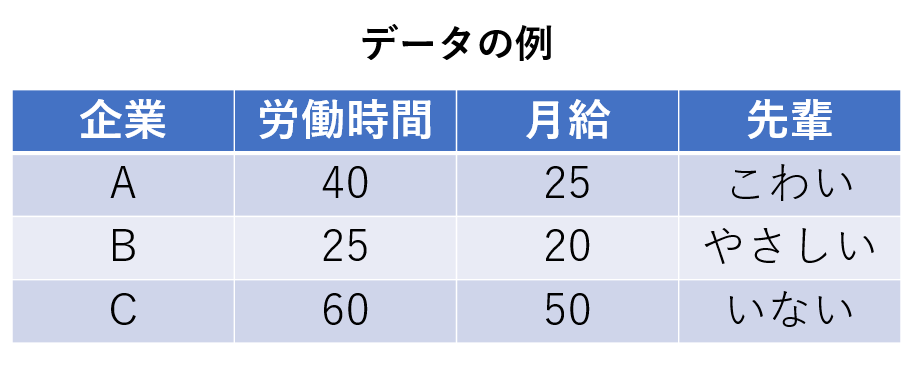
\includegraphics[width=0.7\linewidth]{figs/data_rei} \end{center}

\begin{itemize}
\item
  データを加工する

  \begin{itemize}
  \tightlist
  \item
    欲しい行だけ抜き出す、欲しい列だけ抜き出す
  \item
    元データの情報を使って、分析のための新しい変数を作る
  \item
    例えば、人口50万人以上の都市に1,
    それ以外に0を入れる「大都市ダミー」を作成する
  \end{itemize}
\end{itemize}
\end{block}

\begin{block}{データの要約・可視化}
\protect\hypertarget{ux30c7ux30fcux30bfux306eux8981ux7d04ux53efux8996ux5316}{}
\begin{itemize}
\tightlist
\item
  要約統計量の作成
\end{itemize}

\begin{center}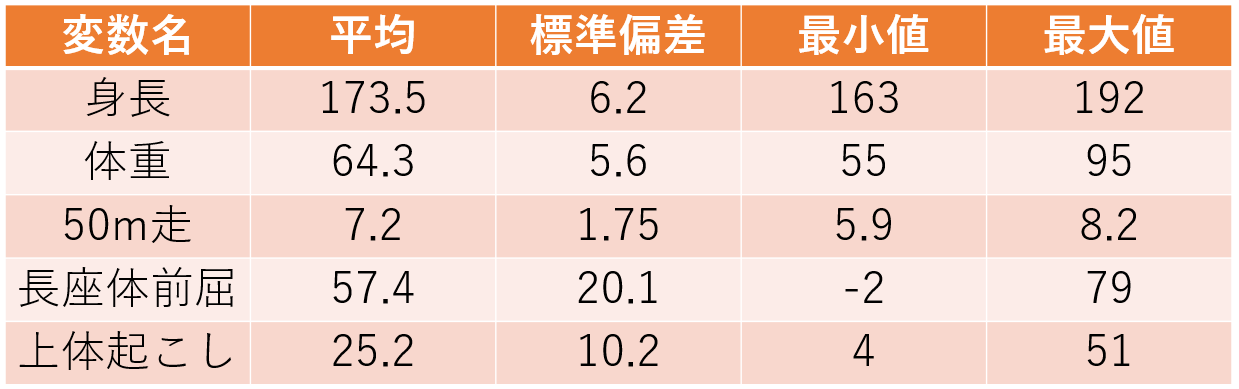
\includegraphics[width=0.8\linewidth]{figs/summary_ex} \end{center}

\begin{itemize}
\tightlist
\item
  データの概要を示す:各変数の平均・標準偏差など
\item
  性別ごと、年代ごとなど、カテゴリで分けて表示する場合も
\item
  可視化できるデータは可視化すると分かりやすい
\end{itemize}
\end{block}

\begin{block}{可視化されたデータの例}
\protect\hypertarget{ux53efux8996ux5316ux3055ux308cux305fux30c7ux30fcux30bfux306eux4f8b}{}
\begin{Shaded}
\begin{Highlighting}[]
\NormalTok{df }\OtherTok{\textless{}{-}}\NormalTok{ palmerpenguins}\SpecialCharTok{::}\NormalTok{penguins}
\NormalTok{ggplot2}\SpecialCharTok{::}\FunctionTok{ggplot}\NormalTok{(df) }\SpecialCharTok{+}
\NormalTok{  ggplot2}\SpecialCharTok{::}\FunctionTok{aes}\NormalTok{(}\AttributeTok{x =}\NormalTok{ body\_mass\_g, }\AttributeTok{y =}\NormalTok{ bill\_length\_mm, }\AttributeTok{fill =}\NormalTok{ species) }\SpecialCharTok{+}
\NormalTok{  ggplot2}\SpecialCharTok{::}\FunctionTok{geom\_point}\NormalTok{(}\AttributeTok{colour =} \StringTok{"black"}\NormalTok{, }\AttributeTok{shape =} \StringTok{"circle filled"}\NormalTok{) }\SpecialCharTok{+}
\NormalTok{  ggplot2}\SpecialCharTok{::}\FunctionTok{scale\_fill\_viridis\_d}\NormalTok{() }\SpecialCharTok{+}
\NormalTok{  ggplot2}\SpecialCharTok{::}\FunctionTok{theme\_bw}\NormalTok{()}
\end{Highlighting}
\end{Shaded}

\begin{center}\includegraphics{introduction1_files/figure-beamer/unnamed-chunk-3-1} \end{center}
\end{block}

\begin{block}{データ分析}
\protect\hypertarget{ux30c7ux30fcux30bfux5206ux6790}{}
\begin{itemize}
\tightlist
\item
  回帰分析などの統計手法による分析を行い、結果をまとめる
\end{itemize}

\[\text{weight}_{i} = \text{flipperSize}_i + \text{Spiecies}_i + u_i\]

\begin{verbatim}
## 
## Call:
## lm(formula = body_mass_g ~ flipper_length_mm + species, data = .)
## 
## Residuals:
##     Min      1Q  Median      3Q     Max 
## -927.70 -254.82  -23.92  241.16 1191.68 
## 
## Coefficients:
##                    Estimate Std. Error t value Pr(>|t|)    
## (Intercept)       -4031.477    584.151  -6.901 2.55e-11 ***
## flipper_length_mm    40.705      3.071  13.255  < 2e-16 ***
## speciesChinstrap   -206.510     57.731  -3.577 0.000398 ***
## speciesGentoo       266.810     95.264   2.801 0.005392 ** 
## ---
## Signif. codes:  0 '***' 0.001 '**' 0.01 '*' 0.05 '.' 0.1 ' ' 1
## 
## Residual standard error: 375.5 on 338 degrees of freedom
##   ( 2 個の観測値が欠損のため削除されました )
## Multiple R-squared:  0.7826, Adjusted R-squared:  0.7807 
## F-statistic: 405.7 on 3 and 338 DF,  p-value: < 2.2e-16
\end{verbatim}
\end{block}

\begin{block}{レポートの作成}
\protect\hypertarget{ux30ecux30ddux30fcux30c8ux306eux4f5cux6210}{}
\begin{itemize}
\tightlist
\item
  Rで行った分析の結果を、Wordやパワーポイントにまとめて出力、保存できる
\item
  習熟度によってはそのまま論文を書くことも可能、そこまでいかずとも色々と手間が省けて便利
\end{itemize}
\end{block}

\begin{block}{おまけ:データの取得}
\protect\hypertarget{ux304aux307eux3051ux30c7ux30fcux30bfux306eux53d6ux5f97}{}
\begin{itemize}
\tightlist
\item
  Rでは様々なデータセットを
\item
  ウェブサイトから情報を収集して分析を行いたい場合がある
\item
  Rのコードからウェブサイトを開き、中の要素を分析に使えるデータセットとして出力することができる
\end{itemize}
\end{block}

\begin{block}{基本構造}
\protect\hypertarget{ux57faux672cux69cbux9020}{}
\begin{itemize}
\item
  基本的には、というか全ての命令は

  \begin{itemize}
  \item
    Rに命令を投げる→命令に従って計算(描画・読み込みなど)を行う
  \item
    必要であればアウトプットを返す
  \end{itemize}

  の繰り返し
\item
  エレベーターの3階ボタンを押す→3階に向かう、ドアを開ける

  \begin{itemize}
  \tightlist
  \item
    ボタンを押すエネルギーでエレベータが動いているわけではない
  \item
    ワイヤーをどれだけ巻き取ればどれだけ上昇・下降するのか、ドアを開けるためにどの部分にどれだけ力を加えればいいのか、が3回ボタンを押したときに発せられる命令として書かれている
  \end{itemize}
\item
  この命令を一つ一つ書く作業を行う
\item
  ExcelやWordなどのソフトウェアでは、こうした命令をコードを書く代わりにボタン操作などでまとめて行ってもらっている
\end{itemize}
\end{block}

\begin{block}{参考}
\protect\hypertarget{ux53c2ux8003}{}
\begin{itemize}
\tightlist
\item
  立命館大:森先生のサイトが大変勉強になります

  \begin{itemize}
  \tightlist
  \item
    \href{https://tomoecon.github.io/R_for_graduate_thesis/}{卒業論文のためのR入門}
  \end{itemize}
\item
  その他、分からないことはgoogleする力を付けましょう

  \begin{itemize}
  \tightlist
  \item
    ``r (関数名)''とかで大体載ってます
  \item
    GitHubなどで自身の作成したライブラリや関数の使い方などを解説しているものも多数存在
  \end{itemize}
\item
  \href{http://cse.naro.affrc.go.jp/takezawa/r-tips/r.html}{R Tips}
\item
  \href{http://www.okadajp.org/RWiki/}{RjpWiki}
\end{itemize}
\end{block}

\begin{block}{その他}
\protect\hypertarget{ux305dux306eux4ed6}{}
\begin{itemize}
\tightlist
\item
  ショートカット:マウスを極力使わない→作業効率の改善
\item
  共通の操作

  \begin{itemize}
  \tightlist
  \item
    Ctrl + X, C, V:順に切り取り・コピー・貼り付け
  \item
    Ctrl + A:全範囲を選択
  \item
    Ctrl + Z, Y:操作を戻す・進める
  \item
    Ctrl + F:ウィンドウ内検索
  \item
    Ctrl + S:(上書き)保存
  \end{itemize}
\item
  R Studio内の操作

  \begin{itemize}
  \tightlist
  \item
    Ctrl + Shift + N:新しいスクリプトを開く
  \item
    Ctrl + O:保存したファイルを開く(Studio以外でもだいたい使える)
  \item
    Ctrl + W:タブを閉じる(Chromeとかブラウザも同じ)
  \item
    Ctrl + Q:R Studioの終了
  \end{itemize}
\item
  Word, PowerPoint, Excelを扱うときもできるだけマウスを使わない

  \begin{itemize}
  \tightlist
  \item
    慣れると作業効率がだいぶ変わる
  \end{itemize}
\end{itemize}
\end{block}
\end{frame}

\begin{frame}[fragile]{Setup}
\protect\hypertarget{setup}{}
\begin{itemize}
\tightlist
\item
  Rでの作業に使うもの

  \begin{itemize}
  \tightlist
  \item
    開発環境とは、R Studioのすすめ
  \end{itemize}
\item
  インストール
\item
  基本操作画面
\end{itemize}

\begin{block}{Rでの作業に必要なもの}
\protect\hypertarget{rux3067ux306eux4f5cux696dux306bux5fc5ux8981ux306aux3082ux306e}{}
\begin{itemize}
\tightlist
\item
  \textbf{R言語}と\textbf{R Studio}の2つをインストール

  \begin{itemize}
  \tightlist
  \item
    R言語をスムーズに利用するためのツール:開発環境がRStudio
  \item
    デフォルトでR GUI
    と呼ばれる開発環境がインストールされるが、色々な理由から使いづらい

    \begin{itemize}
    \tightlist
    \item
      罫線の引いてあるノートに書くか、自由帳に書くかみたいな違い
    \item
      最終的にR言語で命令を書くのは同じ
    \end{itemize}
  \item
    その他にも Jupyter Notebook, VS Code,
    Atomなど様々な開発環境があるので、好きなものを使えばよい
  \end{itemize}
\item
  R Studio Cloud: クラウド上でR Studioの機能を利用できるサービス

  \begin{itemize}
  \tightlist
  \item
    無料の場合は月あたりの利用時間が制限されるなど問題はあるが、特に自前PCのない人は検討してみてもよいかも
  \end{itemize}
\end{itemize}
\end{block}

\begin{block}{RとR Studio}
\protect\hypertarget{rux3068r-studio}{}
\begin{center}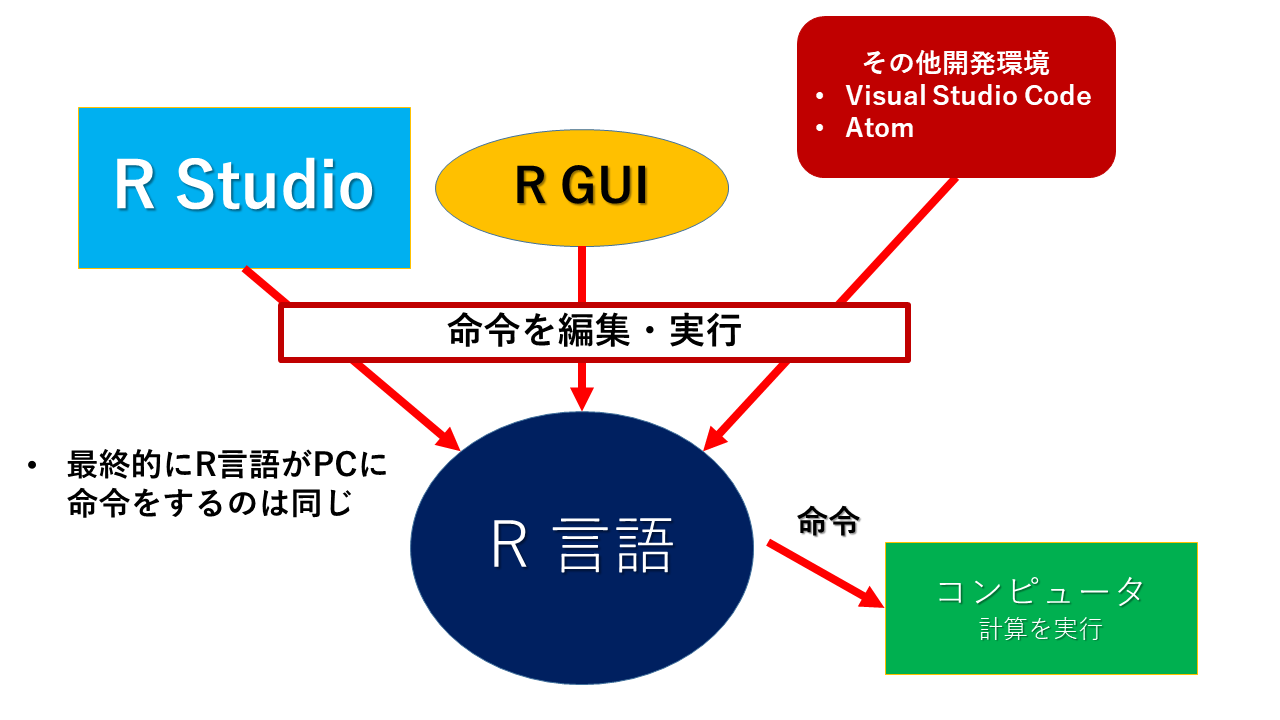
\includegraphics[width=0.95\linewidth]{figs/r_structure} \end{center}
\end{block}

\begin{block}{インストール}
\protect\hypertarget{ux30a4ux30f3ux30b9ux30c8ux30fcux30eb}{}
\href{https://cran.ism.ac.jp/}{Rのダウンロードはここから}

\href{https://www.rstudio.com/products/rstudio/download/\#download}{RStudio
Desktop}

\begin{itemize}
\tightlist
\item
  【定期】詰まったら4回生に訊いて下さい
\item
  それぞれ必ず最新バージョンをダウンロードすること

  \begin{itemize}
  \tightlist
  \item
    定期的にアップデートしておくのがおすすめ、たまに関数の仕様とかが大幅に変わる
  \item
    たぶんいないと思いますが、Ver.4.0.0以前のものを使用している4回生はインストールし直して下さい
  \end{itemize}
\item
  Cドライブに日本語フォントが含まれている人

  \begin{itemize}
  \tightlist
  \item
    C:/Users/\ldots/\ldots のところ
  \item
    ファイルの保存などする際に非常に面倒なことになります
  \item
    特に動作で問題が出なければいいですが、コードの実行中に止まるなどあれば相談して下さい
  \item
    今から買う人は絶対に日本語フォントを入れないようにしましょう、一生
  \end{itemize}
\end{itemize}
\end{block}

\begin{block}{R Studioの基本画面}
\protect\hypertarget{r-studioux306eux57faux672cux753bux9762}{}
\begin{itemize}
\tightlist
\item
  4つの画面 (Pane)が表示される: コードを入力するのは Source,
  Consoleの2つ

  \begin{itemize}
  \tightlist
  \item
    Source:Rスクリプトなどを編集・保存
  \item
    Console:実行するコードを直接入力・実行できる。
  \item
    右側の Pane
    では読み込んだデータフレームやオブジェクトの定義確認、図表出力のチェックなどが行える
  \end{itemize}
\end{itemize}

\begin{center}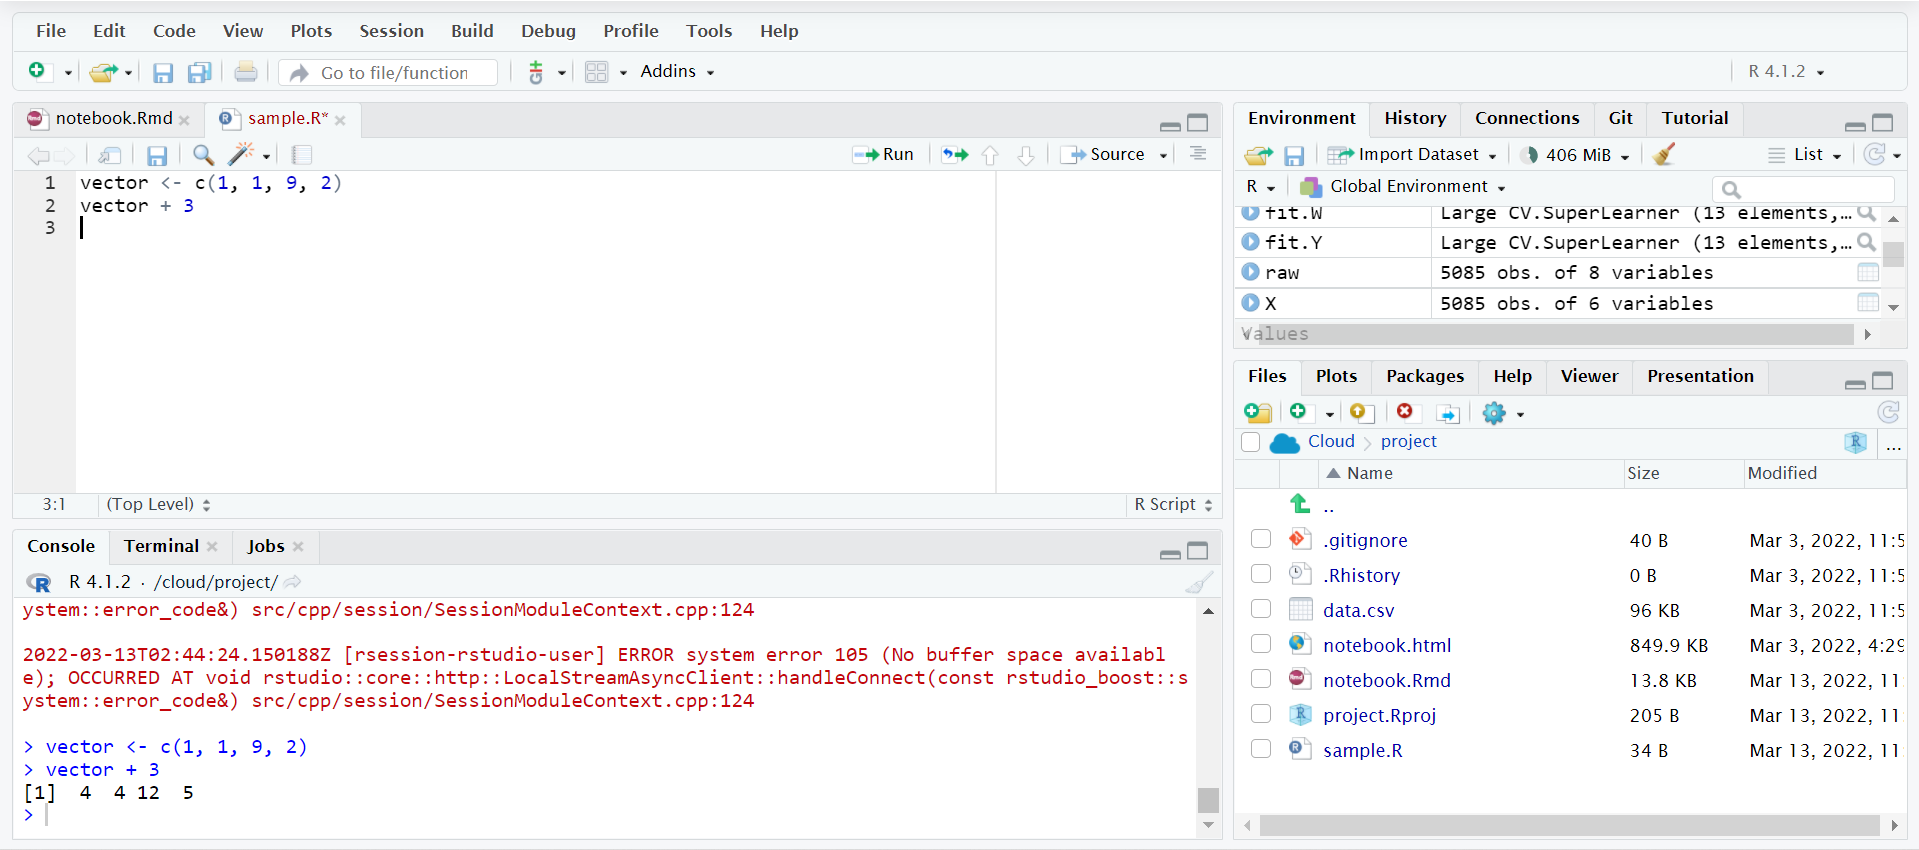
\includegraphics[width=0.77\linewidth]{figs/rstudio_appearance} \end{center}
\end{block}

\begin{block}{触ってみる}
\protect\hypertarget{ux89e6ux3063ux3066ux307fux308b}{}
\begin{itemize}
\tightlist
\item
  コンソールに適当なコードを入力してみよう
\end{itemize}

\begin{Shaded}
\begin{Highlighting}[]
\DecValTok{1} \SpecialCharTok{+} \DecValTok{3} \SpecialCharTok{+} \DecValTok{5}
\end{Highlighting}
\end{Shaded}

\begin{verbatim}
## [1] 9
\end{verbatim}

\begin{itemize}
\tightlist
\item
  コンソールではEnter, ソース(スクリプト)ではCtrl +
  Enterでコードを実行する
\item
  出力は\textgreater に続いて出る(文字色が変わるので分かりやすいはず)
\item
  このスライド上では、コード、出力を四角囲みで、うち出力を\#\#に続く形で表現する
\end{itemize}
\end{block}
\end{frame}

\begin{frame}[fragile]{プロジェクトの作成、バージョン管理}
\protect\hypertarget{ux30d7ux30edux30b8ux30a7ux30afux30c8ux306eux4f5cux6210ux30d0ux30fcux30b8ux30e7ux30f3ux7ba1ux7406}{}
\begin{itemize}
\tightlist
\item
  ディレクトリとは
\item
  ディレクトリの構造
\item
  フォルダの共有方法
\item
  R Studioでプロジェクトを作成する方法
\end{itemize}

\begin{block}{ディレクトリ}
\protect\hypertarget{ux30c7ux30a3ux30ecux30afux30c8ux30ea}{}
\begin{itemize}
\tightlist
\item
  ファイルやフォルダを参照する際に示すPC内の\textbf{住所}

  \begin{itemize}
  \tightlist
  \item
    C:/\ldots がそれ
  \item
    全てが同じ階層に入っているのは作業こそ楽だが、自分で参照するときに探すのが面倒

    \begin{itemize}
    \tightlist
    \item
      ゼミ論文に使うdata.csvというファイルを保存→他の講義で同じ名前のファイルを受け取る→後から見たらどれがどれだか分からなくなる
    \end{itemize}
  \end{itemize}
\item
  整理の方法:
  作業やファイルの種類ごとにフォルダを作り、異なる系統のファイルを識別

  \begin{itemize}
  \tightlist
  \item
    何をする作業のフォルダなのか?
  \item
    データの種類:整理する前の生データなのか、そのまま分析に使えるデータなのか?
  \item
    アウトプット: 分析結果、図表
  \end{itemize}
\item
  R
  Studioでは、特定のフォルダを「プロジェクト」として扱い、「誰のPCでも動くコード」を作ることができる
\end{itemize}
\end{block}

\begin{block}{ディレクトリの構造}
\protect\hypertarget{ux30c7ux30a3ux30ecux30afux30c8ux30eaux306eux69cbux9020}{}
\begin{center}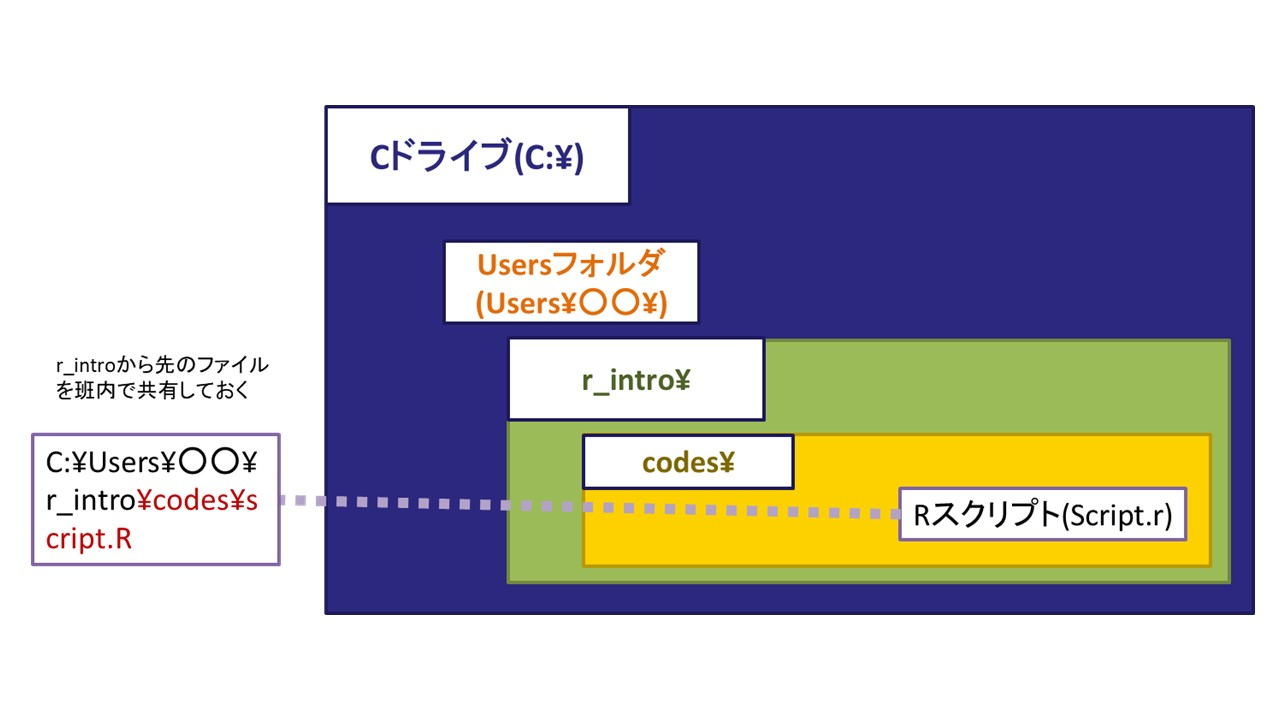
\includegraphics[width=0.77\linewidth]{figs/folder} \end{center}

\begin{itemize}
\tightlist
\item
  使いやすいフォルダの作成

  \begin{itemize}
  \tightlist
  \item
    各自のPCで``r\_intro''フォルダを作り、必要なファイルをしまっておけば、誰が書いたコードでも個々人がPCで再現できる環境に
  \item
    フォルダ名は\textbackslash(バックスラッシュ, ¥)を/
    (スラッシュ)に変えて記述
  \end{itemize}
\end{itemize}
\end{block}

\begin{block}{フォルダ}
\protect\hypertarget{ux30d5ux30a9ux30ebux30c0}{}
\begin{center}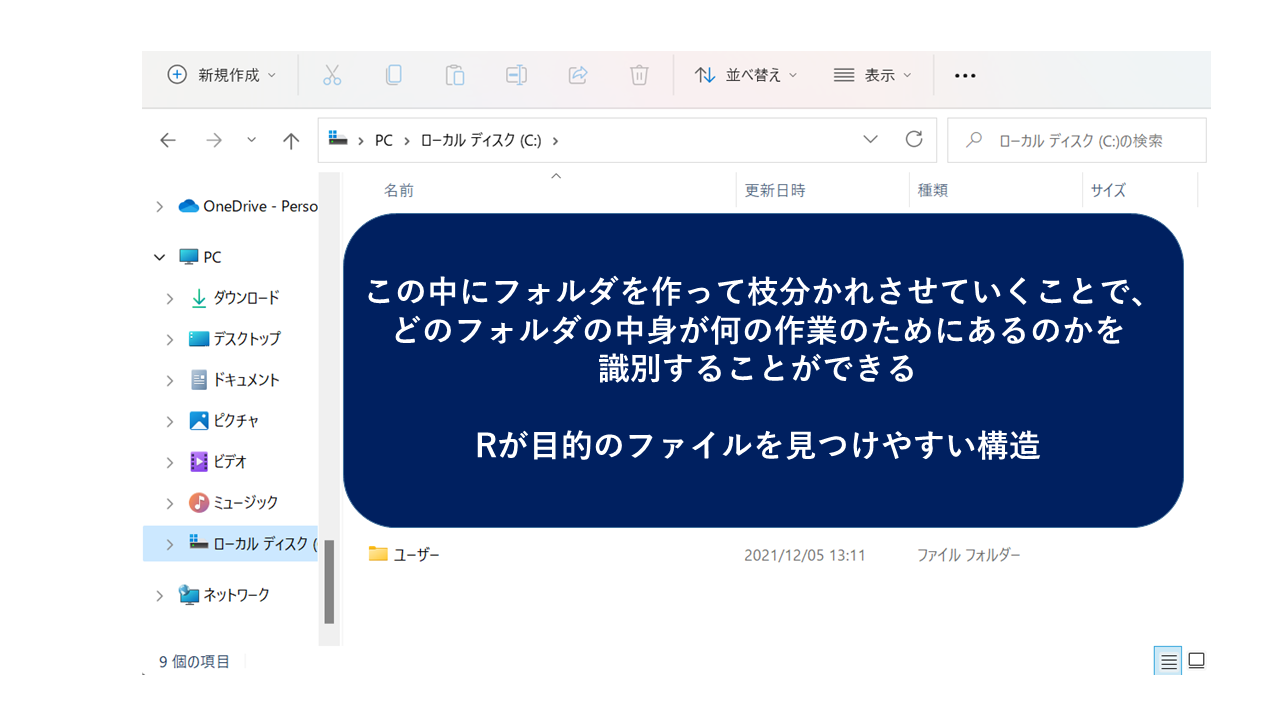
\includegraphics[width=0.95\linewidth]{figs/directory_system} \end{center}
\end{block}

\begin{block}{フォルダ (cont'd)}
\protect\hypertarget{ux30d5ux30a9ux30ebux30c0-contd}{}
\begin{center}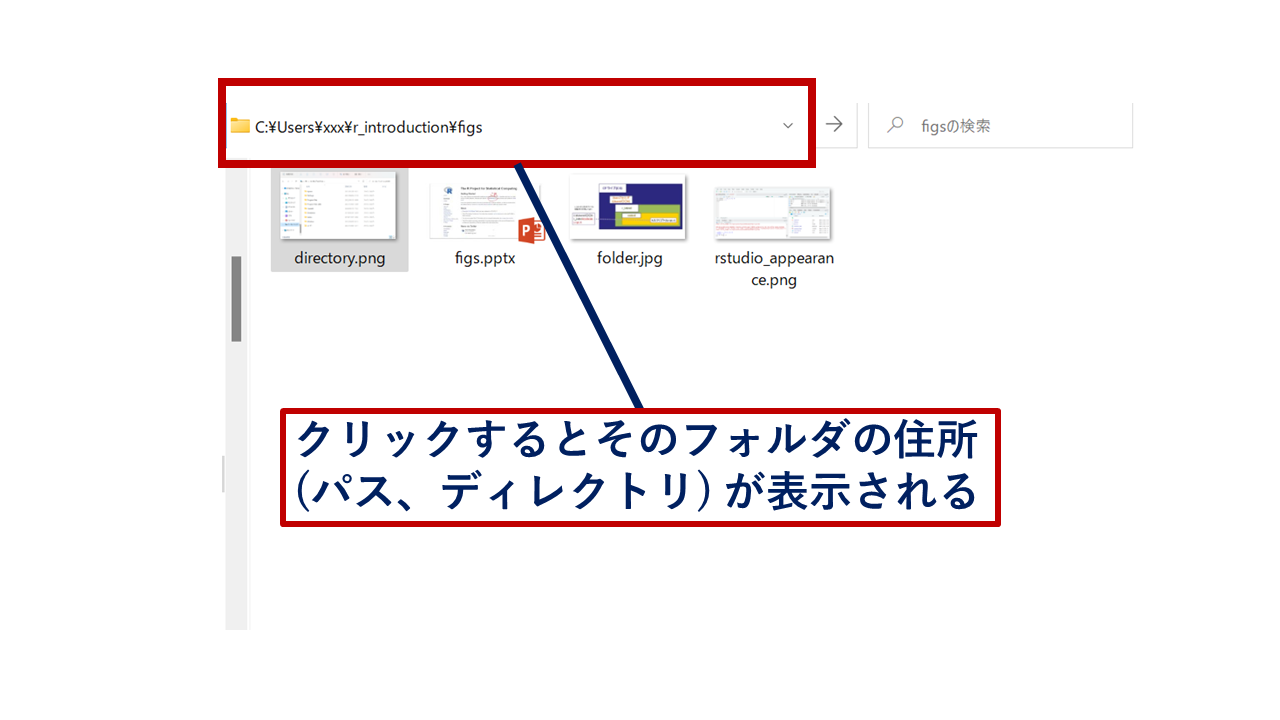
\includegraphics[width=0.95\linewidth]{figs/directory_system2} \end{center}
\end{block}

\begin{block}{ワーキングディレクトリの確認と変更}
\protect\hypertarget{ux30efux30fcux30adux30f3ux30b0ux30c7ux30a3ux30ecux30afux30c8ux30eaux306eux78baux8a8dux3068ux5909ux66f4}{}
\begin{itemize}
\tightlist
\item
  ワーキングディレクトリ:Rが見ているフォルダ

  \begin{itemize}
  \tightlist
  \item
    CSVなどのファイルを読み込む際は、このフォルダから指定された名前のファイルを探す
  \end{itemize}
\item
  R
  Studioのプロジェクトを利用している時は、そのフォルダがある場所がワーキングディレクトリ
\item
  \texttt{getwd}関数で今のワーキングディレクトリを確認できる

  \begin{itemize}
  \tightlist
  \item
    \texttt{setwd}で変更できるが、基本的には相対パスで指定した方が再現性が高いのでおすすめ
  \end{itemize}
\item
  ファイル名:基本全て""で囲む、ワーキングディレクトリの中にあるフォルダを開きたい場合は/で区切る

  \begin{itemize}
  \tightlist
  \item
    \texttt{"C:/folder1/folder2/data.csv"}
  \end{itemize}
\end{itemize}
\end{block}

\begin{block}{拡張子}
\protect\hypertarget{ux62e1ux5f35ux5b50}{}
\begin{itemize}
\tightlist
\item
  PC上で扱うファイルには、それがどのアプリケーション(ソフト)で利用するものなのかがPC側に伝わる印が付いていることが多い:拡張子

  \begin{itemize}
  \tightlist
  \item
    例えば.csvはMicrosoft Excelで開くと決めている(既定のアプリ)
  \item
    .RはRスクリプトを表すことが分かるのでR StudioやR
    GUI、.htmlはブラウザで開く
  \item
    R Studio、Excelのそれぞれでcsvファイルを開いてみよう
  \end{itemize}
\end{itemize}
\end{block}

\begin{block}{フォルダの共有方法}
\protect\hypertarget{ux30d5ux30a9ux30ebux30c0ux306eux5171ux6709ux65b9ux6cd5}{}
\begin{itemize}
\tightlist
\item
  フォルダの共有:データや書いたスクリプトを共有する

  \begin{itemize}
  \tightlist
  \item
    何度も修正を加えたり、作った図表を共有するのはめんどい
  \item
    結果、分析をした人がスライドも全部作る\ldots になりがち
  \end{itemize}
\item
  フォルダをメンバー間で同期する(共有する)ツールをマスターすると、グループでの作業が楽になる

  \begin{itemize}
  \tightlist
  \item
    \href{https://www.dropbox.com/}{Dropbox}
  \item
    \href{https://github.com/}{GitHub}
  \end{itemize}
\item
  特にGitHubはRStudioと直接連携して簡単にクラウド共有・共有したデータのダウンロードも可能なので非常に便利

  \begin{itemize}
  \tightlist
  \item
    データをオープンで保有することになるので、扱うデータの種類によっては注意が必要
  \end{itemize}
\end{itemize}
\end{block}

\begin{block}{フォルダの共有方法(cont'd)}
\protect\hypertarget{ux30d5ux30a9ux30ebux30c0ux306eux5171ux6709ux65b9ux6cd5contd}{}
\begin{itemize}
\tightlist
\item
  Google Driveを使う方法もあり

  \begin{itemize}
  \tightlist
  \item
    Google Document, Spreadsheet, Slides を使った論文共同執筆はべんり
  \item
    OfficeのWord, Excel, Powerpointに比べると機能がかなり制限される弱点
  \item
    特にスライド作成に関しては不便なポイントが多いかも
  \end{itemize}
\item
  文面はGoogle
  Driveで共有しながら作成しつつ、体裁を適宜Wordにダウンロードするなどして修正する必要がある
\end{itemize}
\end{block}

\begin{block}{プロジェクトの作り方}
\protect\hypertarget{ux30d7ux30edux30b8ux30a7ux30afux30c8ux306eux4f5cux308aux65b9}{}
\begin{center}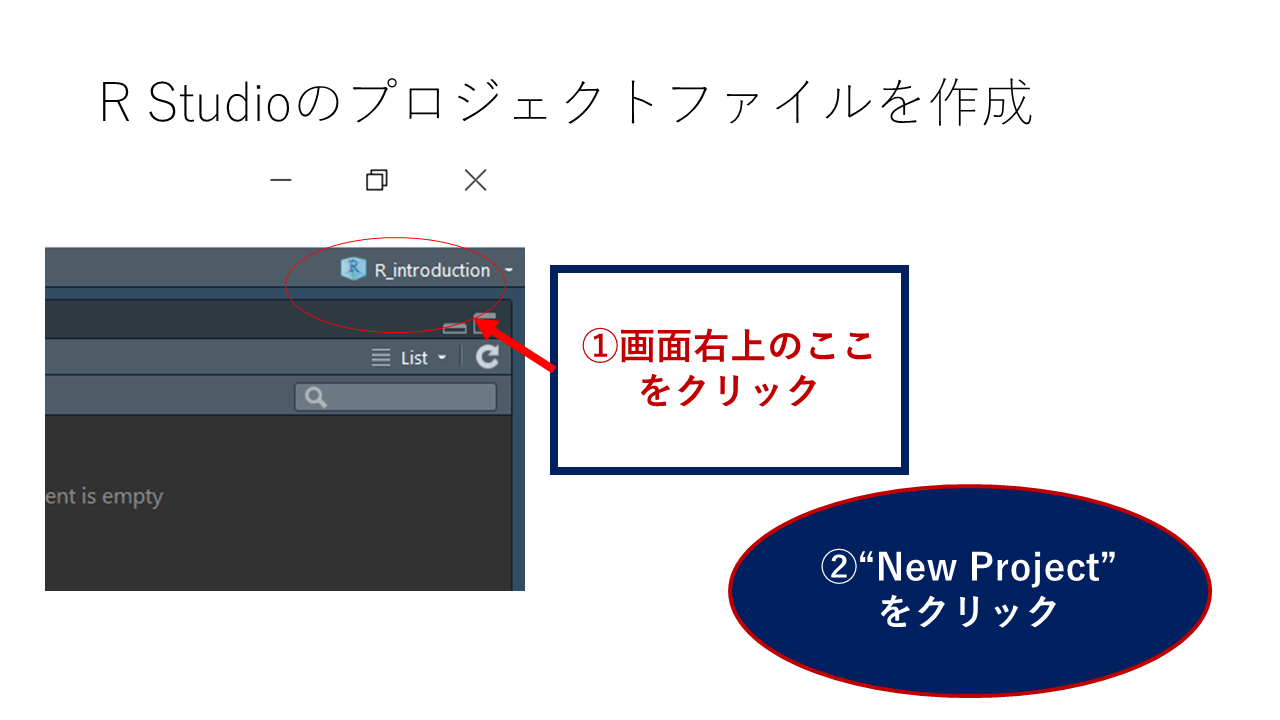
\includegraphics[width=0.95\linewidth]{figs/create_repository} \end{center}
\end{block}

\begin{block}{プロジェクトの作り方(cont'd)}
\protect\hypertarget{ux30d7ux30edux30b8ux30a7ux30afux30c8ux306eux4f5cux308aux65b9contd}{}
\begin{center}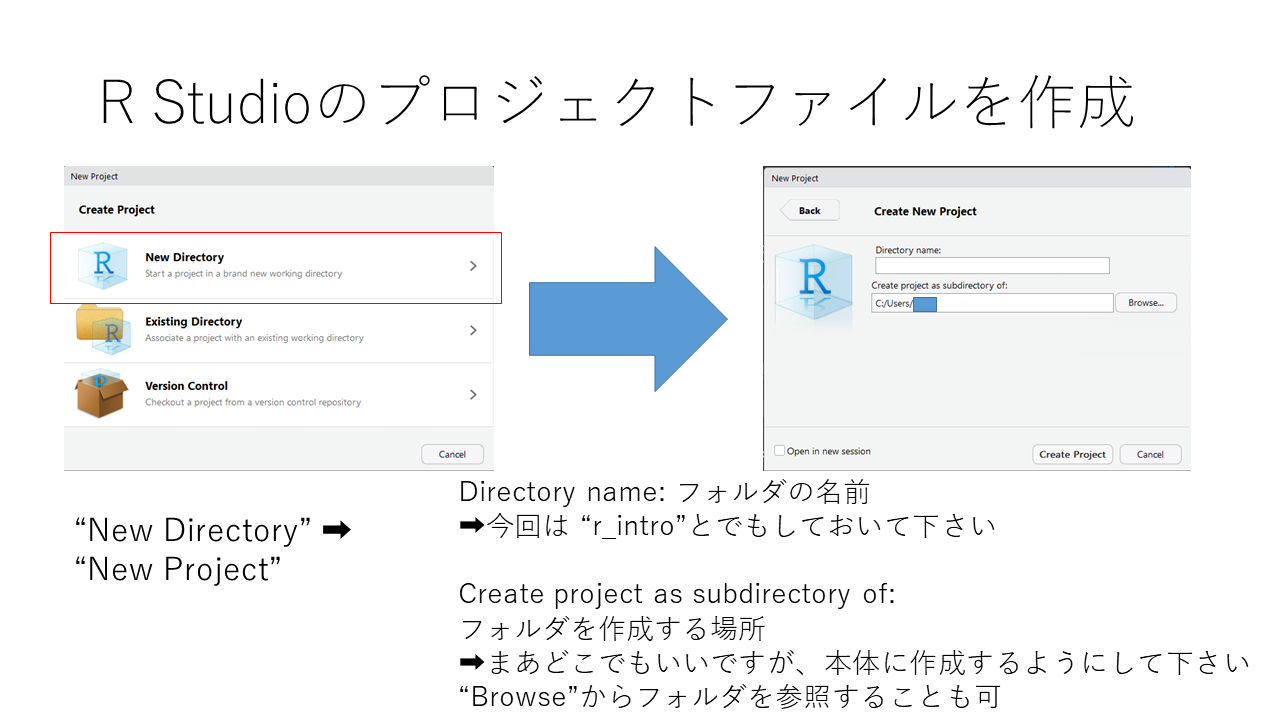
\includegraphics[width=0.95\linewidth]{figs/create_repository2} \end{center}
\end{block}

\begin{block}{ディレクトリの管理}
\protect\hypertarget{ux30c7ux30a3ux30ecux30afux30c8ux30eaux306eux7ba1ux7406}{}
\begin{center}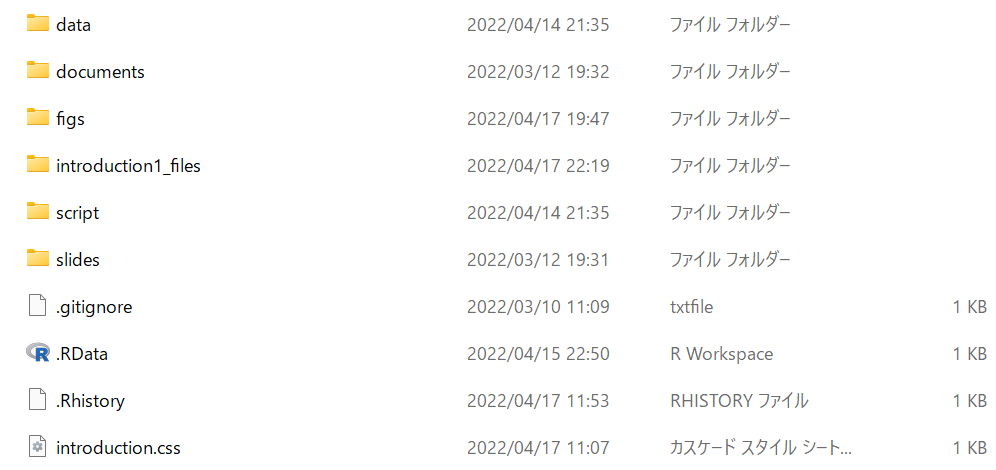
\includegraphics[width=0.95\linewidth]{figs/directory_example} \end{center}

\begin{itemize}
\tightlist
\item
  元データ、Rスクリプト、作成した画像や表\ldots など、作ったものをフォルダで整理すると便利
\item
  とりあえず、作ったプロジェクトフォルダに「data」と「script」のフォルダを作成してみよう
\end{itemize}
\end{block}
\end{frame}

\begin{frame}[fragile]{基本操作}
\protect\hypertarget{ux57faux672cux64cdux4f5c}{}
\begin{itemize}
\tightlist
\item
  コンソールに数値を打ち込む、計算する
\item
  スクリプトの作成
\item
  変数の型
\item
  オブジェクトに数値などを割り当てる
\item
  値を束にして扱う
\end{itemize}

\begin{block}{入力画面}
\protect\hypertarget{ux5165ux529bux753bux9762}{}
\begin{itemize}
\tightlist
\item
  コンソール(通常左下)の``\textgreater{}''が入力待ち状態を表す
\item
  命令を書いてEnterキーを押すと実行できる
\end{itemize}

\begin{center}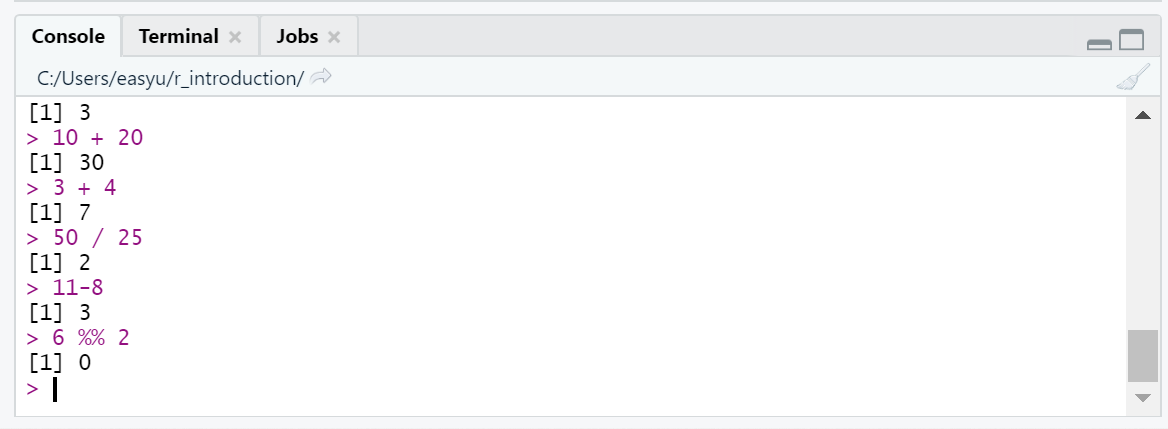
\includegraphics[width=0.95\linewidth]{figs/console} \end{center}
\end{block}

\begin{block}{スクリプトの作成、演算子}
\protect\hypertarget{ux30b9ux30afux30eaux30d7ux30c8ux306eux4f5cux6210ux6f14ux7b97ux5b50}{}
\begin{itemize}
\item
  ``r\_introduction''というプロジェクトを作成
\item
  R Studioを開く

  \begin{itemize}
  \tightlist
  \item
    R
    Consoleにコードを直接入力してEnter、もしくはRスクリプトにコードを記述してCtrl
    + Enterで実行
  \item
    RスクリプトはCtrl+Shift+Nで作成可能
  \item
    Ctrl + Sで保存、上書き保存
  \end{itemize}
\end{itemize}

\begin{Shaded}
\begin{Highlighting}[]
\DecValTok{1} \SpecialCharTok{+} \DecValTok{2} \SpecialCharTok{*}\NormalTok{ (}\DecValTok{3} \SpecialCharTok{/} \DecValTok{4}\NormalTok{) }\CommentTok{\# 掛け算は*で}
\end{Highlighting}
\end{Shaded}

\begin{verbatim}
## [1] 2.5
\end{verbatim}

\begin{itemize}
\tightlist
\item
  その他、基本的な演算記号は\href{http://cse.naro.affrc.go.jp/takezawa/r-tips/r.html}{R-Tips}などを参照
\end{itemize}
\end{block}

\begin{block}{Source: スクリプトやマークダウンファイルの編集}
\protect\hypertarget{source-ux30b9ux30afux30eaux30d7ux30c8ux3084ux30deux30fcux30afux30c0ux30a6ux30f3ux30d5ux30a1ux30a4ux30ebux306eux7de8ux96c6}{}
\begin{center}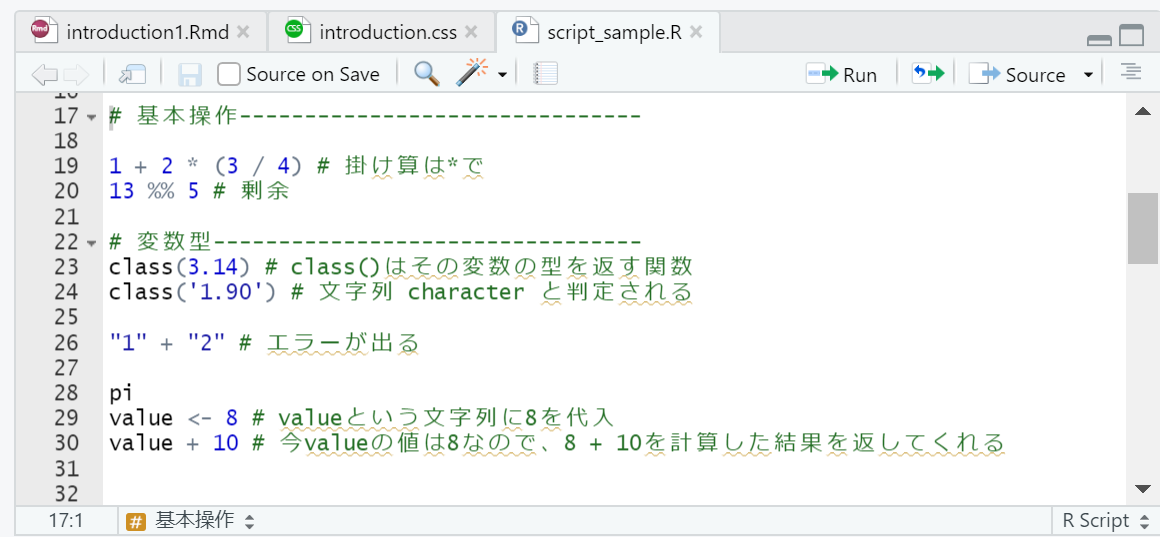
\includegraphics[width=0.95\linewidth]{figs/script} \end{center}

\begin{itemize}
\tightlist
\item
  Ctrl + Enterで選択箇所のコードを実行
\item
  長いコードを途中で改行できることも利点
\item
  Ctrl + Sで適宜上書き保存できる
\end{itemize}
\end{block}

\begin{block}{変数の型}
\protect\hypertarget{ux5909ux6570ux306eux578b}{}
\begin{itemize}
\tightlist
\item
  数値だけでなく、文字も扱うことができる

  \begin{itemize}
  \tightlist
  \item
    何を使っても良いわけではない:Excelも一緒

    \begin{itemize}
    \tightlist
    \item
      電話番号を入力したのに頭の0が消える→Excelが電話番号を数値として認識してしまっているから
    \item
      Excelの場合、数値の形式を標準(Excelに自己判断させる)から文字列に変更することで対処
    \end{itemize}
  \item
    文字列を""で囲って表記することで、それが文字列であることをRに伝えることができる
  \item
    class関数(関数については後述)を使うと、その値の型が分かる
  \end{itemize}
\end{itemize}

\begin{Shaded}
\begin{Highlighting}[]
\FunctionTok{class}\NormalTok{(}\FloatTok{3.14}\NormalTok{) }\CommentTok{\# class()はその変数の型を返す関数}
\end{Highlighting}
\end{Shaded}

\begin{verbatim}
## [1] "numeric"
\end{verbatim}

\begin{Shaded}
\begin{Highlighting}[]
\FunctionTok{class}\NormalTok{(}\StringTok{\textquotesingle{}1.90\textquotesingle{}}\NormalTok{) }\CommentTok{\# 文字列 character と判定される}
\end{Highlighting}
\end{Shaded}

\begin{verbatim}
## [1] "character"
\end{verbatim}
\end{block}

\begin{block}{変数の型(cont'd)}
\protect\hypertarget{ux5909ux6570ux306eux578bcontd}{}
\begin{itemize}
\tightlist
\item
  numeric, integerは足し引きできるが、characterはできない

  \begin{itemize}
  \tightlist
  \item
    integerは整数
  \end{itemize}
\end{itemize}

\begin{Shaded}
\begin{Highlighting}[]
\StringTok{"1"} \SpecialCharTok{+} \StringTok{"2"} \CommentTok{\# エラーが出る}
\end{Highlighting}
\end{Shaded}

\begin{Shaded}
\begin{Highlighting}[]
\FunctionTok{class}\NormalTok{(11L) }\CommentTok{\# 整数の後ろに"L"を付けると整数として認識される}
\end{Highlighting}
\end{Shaded}

\begin{verbatim}
## [1] "integer"
\end{verbatim}
\end{block}

\begin{block}{変数の型(cont'd)}
\protect\hypertarget{ux5909ux6570ux306eux578bcontd-1}{}
\begin{itemize}
\tightlist
\item
  factor

  \begin{itemize}
  \tightlist
  \item
    順序が付いた文字列
  \item
    factor()で定義
  \item
    アルファベット順や数字順以外の方法で並べたい場合に使う
  \item
    まあ使うときにやればいいとおもいます
  \end{itemize}
\end{itemize}

\begin{Shaded}
\begin{Highlighting}[]
\FunctionTok{factor}\NormalTok{(}\FunctionTok{c}\NormalTok{(}\StringTok{"January"}\NormalTok{, }\StringTok{"February"}\NormalTok{, }\StringTok{"March"}\NormalTok{, }\StringTok{"April"}\NormalTok{)) }\CommentTok{\# アルファベット順に並んでしまう}
\end{Highlighting}
\end{Shaded}

\begin{verbatim}
## [1] January  February March    April   
## Levels: April February January March
\end{verbatim}

\begin{Shaded}
\begin{Highlighting}[]
\FunctionTok{factor}\NormalTok{(}\FunctionTok{c}\NormalTok{(}\StringTok{"January"}\NormalTok{, }\StringTok{"February"}\NormalTok{, }\StringTok{"March"}\NormalTok{, }\StringTok{"April"}\NormalTok{), }
       \AttributeTok{levels =} \FunctionTok{c}\NormalTok{(}\StringTok{"January"}\NormalTok{, }\StringTok{"February"}\NormalTok{, }\StringTok{"March"}\NormalTok{, }\StringTok{"April"}\NormalTok{))}
\end{Highlighting}
\end{Shaded}

\begin{verbatim}
## [1] January  February March    April   
## Levels: January February March April
\end{verbatim}
\end{block}

\begin{block}{オブジェクト}
\protect\hypertarget{ux30aaux30d6ux30b8ux30a7ux30afux30c8}{}
\begin{itemize}
\tightlist
\item
  では""で囲わずに入力した文字列はどう認識されるのか?

  \begin{enumerate}
  \tightlist
  \item
    特定の値と結びついている
  \end{enumerate}

  \begin{itemize}
  \tightlist
  \item
    \texttt{pi}: 円周率
  \end{itemize}

  \begin{enumerate}
  \setcounter{enumi}{1}
  \tightlist
  \item
    自信が定義した任意の値が格納されている
  \end{enumerate}

  \begin{itemize}
  \tightlist
  \item
    オブジェクト: 数値やベクトル、データフレームやリストを格納、R
    Studioでは右上のEnvironmentタブに定義が表示される
  \item
    回帰分析などの計算結果を格納することも可能
  \item
    \texttt{\textless{}-} を使って適当な値を定義する
  \item
    \texttt{wani\ \textless{}-\ 3}:waniというオブジェクトに値3を格納
  \end{itemize}
\item
  R Studioでは Environmentに定義したオブジェクトの中身が表示される
\end{itemize}
\end{block}

\begin{block}{オブジェクトの定義}
\protect\hypertarget{ux30aaux30d6ux30b8ux30a7ux30afux30c8ux306eux5b9aux7fa9}{}
\begin{Shaded}
\begin{Highlighting}[]
\NormalTok{pi }\CommentTok{\# デフォルトで円周率が格納されている}
\end{Highlighting}
\end{Shaded}

\begin{verbatim}
## [1] 3.141593
\end{verbatim}

\begin{Shaded}
\begin{Highlighting}[]
\NormalTok{value }\OtherTok{\textless{}{-}} \DecValTok{8} \CommentTok{\# valueという文字列に8を代入}
\NormalTok{value }\SpecialCharTok{+} \DecValTok{10} \CommentTok{\# 今valueの値は8なので、8 + 10を計算した結果を返してくれる}
\end{Highlighting}
\end{Shaded}

\begin{verbatim}
## [1] 18
\end{verbatim}
\end{block}

\begin{block}{値を束にして扱う}
\protect\hypertarget{ux5024ux3092ux675fux306bux3057ux3066ux6271ux3046}{}
\begin{itemize}
\tightlist
\item
  ぶっちゃけ、\(5 \times 5\)ぐらいの計算なら電卓でやればよい
\item
  R、というかPCで計算ができる強みは、複数の計算や結果の保存を同時に行うことができる点

  \begin{itemize}
  \tightlist
  \item
    人間の頭は複数の計算を同時に扱えない
  \item
    計量分析を行う上で不可欠な行列計算などと相性が良い
  \end{itemize}
\item
  Rには複数の数値を扱うための束を作る記法が存在する

  \begin{itemize}
  \tightlist
  \item
    ベクトル:複数の値を順番付きで格納
  \item
    行列、データフレーム:行方向と列方向に展開、ベクトルを束にしたものともいえる
  \item
    リスト:行列やデータフレームを束にして扱うことができる
  \end{itemize}
\end{itemize}
\end{block}

\begin{block}{ベクトル}
\protect\hypertarget{ux30d9ux30afux30c8ux30eb}{}
\begin{itemize}
\tightlist
\item
  ベクトル:複数の要素を含む列

  \begin{itemize}
  \tightlist
  \item
    \texttt{c(a,\ b,\ c,\ ...)}で定義される
  \item
    文字列など、他の数値型を利用してもOK
  \end{itemize}
\end{itemize}

\begin{Shaded}
\begin{Highlighting}[]
\NormalTok{vec }\OtherTok{\textless{}{-}} \FunctionTok{c}\NormalTok{(}\DecValTok{1192}\NormalTok{, }\DecValTok{2960}\NormalTok{)}
\NormalTok{vec }\SpecialCharTok{*} \DecValTok{2}
\end{Highlighting}
\end{Shaded}

\begin{verbatim}
## [1] 2384 5920
\end{verbatim}

\begin{itemize}
\tightlist
\item
  関数(後述)を用いて規則性のあるベクトルを簡単に定義することもできる

  \begin{itemize}
  \tightlist
  \item
    \texttt{seq(a,\ b,\ c)}: aからbまで、公差cの等差数列

    \begin{itemize}
    \tightlist
    \item
      公差が1の場合は、\texttt{a:b}でも代替可能
    \end{itemize}
  \item
    \texttt{rep(a,\ b)}: aをb回繰り返す数列
  \end{itemize}
\end{itemize}

\begin{Shaded}
\begin{Highlighting}[]
\FunctionTok{seq}\NormalTok{(}\DecValTok{1}\NormalTok{, }\DecValTok{10}\NormalTok{, }\DecValTok{2}\NormalTok{)}
\end{Highlighting}
\end{Shaded}

\begin{verbatim}
## [1] 1 3 5 7 9
\end{verbatim}
\end{block}

\begin{block}{データフレーム}
\protect\hypertarget{ux30c7ux30fcux30bfux30d5ux30ecux30fcux30e0}{}
\begin{itemize}
\item
  各行に観測単位(個人、グループ、都道府県など)、各列に特定の情報を含んだデータ形式

  \begin{itemize}
  \tightlist
  \item
    実際にデータ分析を行う際は、csvファイルなどをこの形式で読み込むことでRで扱えるようにする
  \end{itemize}
\item
  100人の性別、学年、学部が分かるデータフレーム:100行×3列のデータフレームになる
\item
  データフレームは\texttt{data.frame}関数、もしくはtibbleパッケージの\texttt{tibble}関数で定義する
\end{itemize}
\end{block}

\begin{block}{データフレーム (cont'd)}
\protect\hypertarget{ux30c7ux30fcux30bfux30d5ux30ecux30fcux30e0-contd}{}
\begin{Shaded}
\begin{Highlighting}[]
\NormalTok{df }\OtherTok{\textless{}{-}} \FunctionTok{data.frame}\NormalTok{( }\CommentTok{\# dfというオブジェクトにデータフレームを定義}
  \AttributeTok{faculty =} \FunctionTok{c}\NormalTok{(}\StringTok{"econ"}\NormalTok{, }\StringTok{"law"}\NormalTok{, }\StringTok{"foreign"}\NormalTok{, }\StringTok{"lit"}\NormalTok{), }\CommentTok{\# 各列のデータをベクトル形式で代入}
  \AttributeTok{grade =} \FunctionTok{c}\NormalTok{(}\DecValTok{4}\NormalTok{, }\DecValTok{2}\NormalTok{, }\DecValTok{1}\NormalTok{, }\DecValTok{1}\NormalTok{),}
  \AttributeTok{toeic =} \FunctionTok{c}\NormalTok{(}\DecValTok{300}\NormalTok{, }\DecValTok{820}\NormalTok{, }\ConstantTok{NA}\NormalTok{, }\DecValTok{785}\NormalTok{) }\CommentTok{\# NA: 該当する値が存在しないことを表す=無回答など}
\NormalTok{)}
\FunctionTok{print}\NormalTok{(df)}
\end{Highlighting}
\end{Shaded}

\begin{verbatim}
##   faculty grade toeic
## 1    econ     4   300
## 2     law     2   820
## 3 foreign     1    NA
## 4     lit     1   785
\end{verbatim}
\end{block}

\begin{block}{定義したデータフレームの確認}
\protect\hypertarget{ux5b9aux7fa9ux3057ux305fux30c7ux30fcux30bfux30d5ux30ecux30fcux30e0ux306eux78baux8a8d}{}
\begin{center}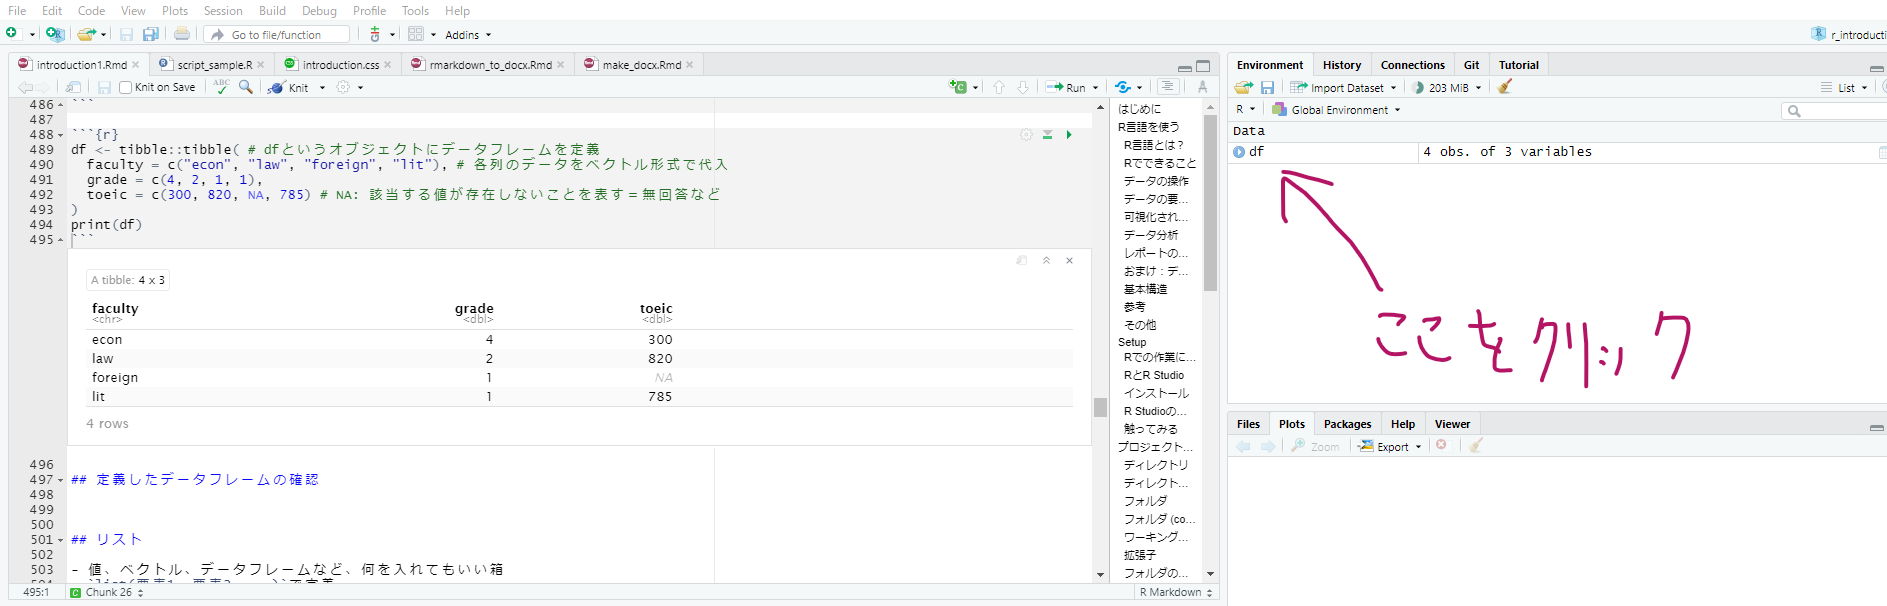
\includegraphics[width=0.9\linewidth]{figs/df_check} \end{center}
\end{block}

\begin{block}{リスト}
\protect\hypertarget{ux30eaux30b9ux30c8}{}
\begin{itemize}
\tightlist
\item
  値、ベクトル、データフレームなど、何を入れてもいい箱
\item
  \texttt{list(要素1,\ 要素2,\ ...)}で定義
\item
  複数のデータフレームに対して同じ操作をしたい場合などに便利
\end{itemize}

\begin{Shaded}
\begin{Highlighting}[]
\NormalTok{listA }\OtherTok{\textless{}{-}} \FunctionTok{list}\NormalTok{(}\FunctionTok{data.frame}\NormalTok{(}\AttributeTok{a =} \DecValTok{1}\SpecialCharTok{:}\DecValTok{5}\NormalTok{, }\AttributeTok{b =} \DecValTok{11}\SpecialCharTok{:}\DecValTok{15}\NormalTok{, }\AttributeTok{c =} \DecValTok{100}\SpecialCharTok{:}\DecValTok{104}\NormalTok{), df)}
\FunctionTok{print}\NormalTok{(listA)}
\end{Highlighting}
\end{Shaded}

\begin{verbatim}
## [[1]]
##   a  b   c
## 1 1 11 100
## 2 2 12 101
## 3 3 13 102
## 4 4 14 103
## 5 5 15 104
## 
## [[2]]
##   faculty grade toeic
## 1    econ     4   300
## 2     law     2   820
## 3 foreign     1    NA
## 4     lit     1   785
\end{verbatim}
\end{block}

\begin{block}{リスト (cont'd)}
\protect\hypertarget{ux30eaux30b9ux30c8-contd}{}
\begin{Shaded}
\begin{Highlighting}[]
\FunctionTok{print}\NormalTok{(listA[[}\DecValTok{1}\NormalTok{]]) }\CommentTok{\# リストの中の一部の要素のみ利用する場合は、[[]]で指定する}
\end{Highlighting}
\end{Shaded}

\begin{verbatim}
##   a  b   c
## 1 1 11 100
## 2 2 12 101
## 3 3 13 102
## 4 4 14 103
## 5 5 15 104
\end{verbatim}

\begin{itemize}
\tightlist
\item
  あんまり便利さが伝わらなさそうなので分析パートで後述
\end{itemize}
\end{block}

\begin{block}{関数}
\protect\hypertarget{ux95a2ux6570}{}
\begin{itemize}
\tightlist
\item
  Rで行う典型的な操作・計算を行う命令
\item
  操作を実行する対象となる値や、実行にあたって選択可能な様々なオプションを(関数名)(引数1
  = ., 引数2 = ., \ldots)の形で記述
\end{itemize}

\begin{Shaded}
\begin{Highlighting}[]
\FunctionTok{log}\NormalTok{(}\AttributeTok{x =} \DecValTok{100}\NormalTok{, }\AttributeTok{base =} \DecValTok{10}\NormalTok{) }\CommentTok{\# 100の対数、底10で計算}
\end{Highlighting}
\end{Shaded}

\begin{verbatim}
## [1] 2
\end{verbatim}

\begin{Shaded}
\begin{Highlighting}[]
\FunctionTok{log}\NormalTok{(}\AttributeTok{x =} \DecValTok{100}\NormalTok{, }\AttributeTok{base =} \DecValTok{5}\NormalTok{) }\CommentTok{\# 底を5に変更}
\end{Highlighting}
\end{Shaded}

\begin{verbatim}
## [1] 2.861353
\end{verbatim}
\end{block}

\begin{block}{関数 (cont'd)}
\protect\hypertarget{ux95a2ux6570-contd}{}
\begin{itemize}
\tightlist
\item
  各関数において使用される引数の名前は決まっており、必要なオプションに対して一つひとつ情報を指定する

  \begin{itemize}
  \tightlist
  \item
    引数には数値や文字列を取ったり、ベクトルやデータフレームを取る時もある
  \end{itemize}
\item
  引数を指定しなければエラーが出るものと、指定しない場合のオプションを自動で選んでくれるものとが存在
\item
  パッケージ名::関数名()でその関数がどのパッケージに属しているかを明示することもできる
\item
  実行結果のエラー

  \begin{itemize}
  \tightlist
  \item
    エラー:引数指定の不備などで計算が実行できなかった場合
  \item
    警告(warning):引数を自動補完した、計算結果に不備があるなどしたが、とりあえず結果は出た
  \end{itemize}
\end{itemize}
\end{block}

\begin{block}{関数とベクトル}
\protect\hypertarget{ux95a2ux6570ux3068ux30d9ux30afux30c8ux30eb}{}
\begin{itemize}
\tightlist
\item
  関数の引数にベクトルやデータフレームを使用するのももちろん可能
\item
  \texttt{mean}関数、\texttt{sd}関数は、それぞれ値の平均、標準偏差を計算する関数
\end{itemize}

\begin{Shaded}
\begin{Highlighting}[]
\NormalTok{values }\OtherTok{\textless{}{-}} \FunctionTok{c}\NormalTok{(}\DecValTok{1}\SpecialCharTok{:}\DecValTok{5}\NormalTok{, }\FunctionTok{rep}\NormalTok{(}\DecValTok{3}\NormalTok{, }\DecValTok{10}\NormalTok{), }\DecValTok{4}\SpecialCharTok{:}\DecValTok{10}\NormalTok{) }\CommentTok{\#1, 2, ..., 5, 3, 3, ... }
\FunctionTok{mean}\NormalTok{(values) }\CommentTok{\# ベクトルの平均を計算}
\end{Highlighting}
\end{Shaded}

\begin{verbatim}
## [1] 4.272727
\end{verbatim}

\begin{Shaded}
\begin{Highlighting}[]
\FunctionTok{sd}\NormalTok{(values)}
\end{Highlighting}
\end{Shaded}

\begin{verbatim}
## [1] 2.333643
\end{verbatim}
\end{block}

\begin{block}{パッケージの利用}
\protect\hypertarget{ux30d1ux30c3ux30b1ux30fcux30b8ux306eux5229ux7528}{}
\begin{itemize}
\tightlist
\item
  パッケージ:便利な関数をまとめて利用可能にする関数のセット
\item
  世界中のプログラマーが様々な分野における分析やデータ収集に関するパッケージを開発・公開している

  \begin{itemize}
  \tightlist
  \item
    これらを全て無料でダウンロードし、利用できるのがRの強み
  \end{itemize}
\item
  \texttt{install.packages}関数を用いてCRAN(公式のインストールサイト)からインストール
\item
  その他、Githubにパッケージを公開している人もいるので、その場合は別の関数を利用
\item
  インストールしたパッケージは、毎回Rの起動時に\texttt{library}関数、もしくは\texttt{require}関数を用いて有効化する
\end{itemize}

\begin{Shaded}
\begin{Highlighting}[]
\FunctionTok{install.packages}\NormalTok{(}\StringTok{"tidyverse"}\NormalTok{) }\CommentTok{\# tidyverse パッケージをインストール}
\FunctionTok{library}\NormalTok{(tidyverse) }\CommentTok{\# tidyverse パッケージを有効化:起動したときに毎回実行する}
\end{Highlighting}
\end{Shaded}
\end{block}

\begin{block}{例:図形の描画}
\protect\hypertarget{ux4f8bux56f3ux5f62ux306eux63cfux753b}{}
\begin{itemize}
\tightlist
\item
  \(y = x^2\)のグラフの描画、定義域は-5から5
\item
  pchはプロットの形を指定、colはプロットの色
\end{itemize}

\begin{Shaded}
\begin{Highlighting}[]
\NormalTok{graphics}\SpecialCharTok{::}\FunctionTok{plot}\NormalTok{(}\AttributeTok{x =} \SpecialCharTok{{-}}\DecValTok{5}\SpecialCharTok{:}\DecValTok{5}\NormalTok{, }\AttributeTok{y =}\NormalTok{ (}\SpecialCharTok{{-}}\DecValTok{5}\SpecialCharTok{:}\DecValTok{5}\NormalTok{)}\SpecialCharTok{\^{}}\DecValTok{2}\NormalTok{, }\AttributeTok{pch =} \DecValTok{19}\NormalTok{, }\AttributeTok{col =} \StringTok{"magenta"}\NormalTok{) }
\end{Highlighting}
\end{Shaded}

\begin{center}\includegraphics[width=0.47\linewidth]{introduction1_files/figure-beamer/unnamed-chunk-28-1} \end{center}
\end{block}
\end{frame}

\begin{frame}[fragile]{データ操作}
\protect\hypertarget{ux30c7ux30fcux30bfux64cdux4f5c}{}
\begin{itemize}
\tightlist
\item
  tidyverse パッケージの活用
\item
  R内のデータセットを利用する
\item
  データの中身を確認する
\item
  csvファイルの読み込み、保存

  \begin{itemize}
  \tightlist
  \item
    csvファイルを保存する
  \item
    PCに保存したデータを読み込む
  \item
    ネットで公開されているcsvファイルを読み込む
  \item
    その他のデータ形式
  \end{itemize}
\item
  データの詳細を調べる

  \begin{itemize}
  \tightlist
  \item
    サイトの参照
  \item
    要約統計量の作成:データの概観を掴む
  \end{itemize}
\item
  データを操作する

  \begin{itemize}
  \tightlist
  \item
    不要な行・列の削除
  \item
    サンプルの分割
  \item
    新しい列の作成・条件分岐
  \item
    文字列の処理
  \end{itemize}
\end{itemize}

\begin{block}{tidyverse パッケージ}
\protect\hypertarget{tidyverse-ux30d1ux30c3ux30b1ux30fcux30b8}{}
\begin{itemize}
\tightlist
\item
  外部からのデータの読み込みや整理、可視化(次章で説明)に必要な関数を一通り揃えた便利なパッケージ
\item
  パッケージの中に様々な目的で作成された複数のパッケージを含んでおり、実際に使用する時は\texttt{library(tidyverse)}で全ての関数を利用できる

  \begin{itemize}
  \tightlist
  \item
    readr: データの読み込みや書き出しを担当するパッケージ
  \item
    ggplot2: データの可視化:散布図やグラフの作成
  \item
    dplyr: データの整形を行うパッケージ
  \item
    purrr: 繰り返し計算(ループ)を行うための関数
  \end{itemize}
\item
  \texttt{install.package}を活用してインストール
\end{itemize}

\begin{Shaded}
\begin{Highlighting}[]
\FunctionTok{install.packages}\NormalTok{(}\StringTok{"tidyverse"}\NormalTok{)}
\FunctionTok{library}\NormalTok{(tidyverse)}
\end{Highlighting}
\end{Shaded}
\end{block}

\begin{block}{パイプ演算子について}
\protect\hypertarget{ux30d1ux30a4ux30d7ux6f14ux7b97ux5b50ux306bux3064ux3044ux3066}{}
\begin{itemize}
\tightlist
\item
  パイプ演算子:\texttt{\%\textgreater{}\%}で記述
\item
  一つのオブジェクト
  (多くはデータフレーム)について、複数の関数を連続して使用したい場合に活用
\item
  関数1 \texttt{\%\textgreater{}\%} 関数2 \texttt{\%\textgreater{}\%}
  関数3\ldots のように記述

  \begin{itemize}
  \tightlist
  \item
    中身は関数3(関数2(関数1))と同じ
  \end{itemize}
\end{itemize}

\begin{Shaded}
\begin{Highlighting}[]
\DecValTok{1}\SpecialCharTok{:}\DecValTok{10} \SpecialCharTok{\%\textgreater{}\%} \CommentTok{\# ベクトルを作る、これが直後の関数で操作される}
  \FunctionTok{mean}\NormalTok{() }\SpecialCharTok{\%\textgreater{}\%} \CommentTok{\# 平均を求める}
  \FunctionTok{print}\NormalTok{() }\CommentTok{\# 計算結果(求めた平均を表示する)}
\end{Highlighting}
\end{Shaded}

\begin{verbatim}
## [1] 5.5
\end{verbatim}

\begin{itemize}
\tightlist
\item
  より直感的に分かりやすいコードが書ける
\item
  計算過程をいちいち他のオブジェクトに置かなくていい
\end{itemize}
\end{block}

\begin{block}{データの取得}
\protect\hypertarget{ux30c7ux30fcux30bfux306eux53d6ux5f97}{}
\begin{itemize}
\tightlist
\item
  分析方法が決まったらデータを取得
\item
  ここではRで簡単に利用できるサンプルデータを取得して分析・可視化を行う
\item
  palmerpenguinsパッケージをインストール、penguins\_rawデータを使ってみる
\end{itemize}

\begin{Shaded}
\begin{Highlighting}[]
\FunctionTok{install.packages}\NormalTok{(}\StringTok{"palmerpenguins"}\NormalTok{)}
\end{Highlighting}
\end{Shaded}

\begin{itemize}
\tightlist
\item
  パッケージを読み込むとデータセットが利用できるようになる
\end{itemize}

\begin{Shaded}
\begin{Highlighting}[]
\FunctionTok{library}\NormalTok{(palmerpenguins)}
\NormalTok{palmerpenguins}\SpecialCharTok{::}\NormalTok{penguins}
\end{Highlighting}
\end{Shaded}

\begin{itemize}
\tightlist
\item
  ``::''の前にパッケージ名、後ろに関数名(or
  データフレーム名)を置く記法ならどのパッケージを利用しているのか分かりやすい、この辺はお好みで
\end{itemize}
\end{block}

\begin{block}{データを確認}
\protect\hypertarget{ux30c7ux30fcux30bfux3092ux78baux8a8d}{}
\includegraphics[width=0.6\linewidth,height=0.6\textheight]{introduction1_files/figure-beamer/unnamed-chunk-33-1}

\begin{itemize}
\tightlist
\item
  penguinデータの他、経済学向けのデータセットも利用できる
\item
  AERパッケージをダウンロードすると良い
\end{itemize}
\end{block}

\begin{block}{Penguins データの概要}
\protect\hypertarget{penguins-ux30c7ux30fcux30bfux306eux6982ux8981}{}
\begin{itemize}
\tightlist
\item
  ペンギンをとっ捕まえて大きさや重さを計測したデータ
\item
  元論文:\href{https://journals.plos.org/plosone/article?id=10.1371/journal.pone.0090081}{Kristen
  B. Gorman ,Tony D. Williams, and William R. Fraser (2014)}
\item
  論文引用のフォーマット

  \begin{itemize}
  \tightlist
  \item
    Gorman KB, Williams TD, Fraser WR (2014) Ecological Sexual
    Dimorphism and Environmental Variability within a Community of
    Antarctic Penguins (Genus Pygoscelis). PLoS ONE 9(3): e90081.
    {[}\url{https://doi.org/10.1371/journal.pone.0090081}{]}
  \item
    著者名、公刊年度、タイトル、学術誌名、その他(URLなど)の順で記載するのが一般的
  \item
    ``Cite''
    みたいなボタンを押すと簡単にフォーマットをコピーできることが多いです
  \end{itemize}
\item
  ここではこのデータセットを例に、基本的なデータ操作を学習する
\item
  palmerpenguinsパッケージには、成型前のデータ(penguins\_raw)も入っている
\end{itemize}
\end{block}

\begin{block}{データの一部分を確認する}
\protect\hypertarget{ux30c7ux30fcux30bfux306eux4e00ux90e8ux5206ux3092ux78baux8a8dux3059ux308b}{}
\begin{itemize}
\tightlist
\item
  head(データフレーム, 行数)でデータの行頭を表示させることができる
\item
  tailなら下から
\end{itemize}

\begin{Shaded}
\begin{Highlighting}[]
\FunctionTok{head}\NormalTok{(penguins\_raw, }\DecValTok{5}\NormalTok{)}
\end{Highlighting}
\end{Shaded}

\begin{verbatim}
## # A tibble: 5 x 17
##   studyName `Sample Number` Species          Region Island Stage `Individual ID`
##   <chr>               <dbl> <chr>            <chr>  <chr>  <chr> <chr>          
## 1 PAL0708                 1 Adelie Penguin ~ Anvers Torge~ Adul~ N1A1           
## 2 PAL0708                 2 Adelie Penguin ~ Anvers Torge~ Adul~ N1A2           
## 3 PAL0708                 3 Adelie Penguin ~ Anvers Torge~ Adul~ N2A1           
## 4 PAL0708                 4 Adelie Penguin ~ Anvers Torge~ Adul~ N2A2           
## 5 PAL0708                 5 Adelie Penguin ~ Anvers Torge~ Adul~ N3A1           
## # ... with 10 more variables: `Clutch Completion` <chr>, `Date Egg` <date>,
## #   `Culmen Length (mm)` <dbl>, `Culmen Depth (mm)` <dbl>,
## #   `Flipper Length (mm)` <dbl>, `Body Mass (g)` <dbl>, Sex <chr>,
## #   `Delta 15 N (o/oo)` <dbl>, `Delta 13 C (o/oo)` <dbl>, Comments <chr>
\end{verbatim}

\begin{itemize}
\tightlist
\item
  R
  Studio中では\texttt{View}関数を使うと別ウインドウで開くのでこれが見やすい
\end{itemize}
\end{block}

\begin{block}{外部ファイルでのデータの扱い}
\protect\hypertarget{ux5916ux90e8ux30d5ux30a1ux30a4ux30ebux3067ux306eux30c7ux30fcux30bfux306eux6271ux3044}{}
\begin{itemize}
\tightlist
\item
  Rで利用できるデータセットはチュートリアルに便利だが、実証分析にそのまま使うのは難しい

  \begin{itemize}
  \tightlist
  \item
    データの種類

    \begin{itemize}
    \tightlist
    \item
      二次データ:官庁や大学、民間のリサーチ会社やデータサイトなど、自分以外が作成したデータを借りる(目的に合うデータがあればこちらがベター)
    \item
      一次データ:自作のアンケートや経済実験などを実施し、自らデータセットを作成する
    \end{itemize}
  \item
    いずれにせよ、外部から取得してきたデータをRに読み込んでもらう必要がある
  \item
    csv (comma separated values)
    ファイルは、代表的なデータ保存方法:データがカンマで区切られている
  \end{itemize}
\item
  ただし、取得したデータにはノイズ(欠損値がある観測や、質問を誤解している回答など)が含まれており、分析を行うためにこれらの問題に対処する必要がある

  \begin{itemize}
  \tightlist
  \item
    分析の種類によっては必要ない情報が含まれていることも
  \item
    データを読み込むと同時に、整理したものを保存しておく機能も必要
  \end{itemize}
\end{itemize}
\end{block}

\begin{block}{取得したデータをcsvファイルとして保存}
\protect\hypertarget{ux53d6ux5f97ux3057ux305fux30c7ux30fcux30bfux3092csvux30d5ux30a1ux30a4ux30ebux3068ux3057ux3066ux4fddux5b58}{}
\begin{itemize}
\tightlist
\item
  \texttt{readr::write\_excel\_csv}関数を活用

  \begin{itemize}
  \tightlist
  \item
    保存したいデータフレーム名と、保存先のファイル名を指定、実行すれば、ファイルをcsv形式で保存してくれる
  \item
    保存したものをExcelで開くことも可能
  \end{itemize}
\item
  プロジェクトファイル内に``data''というフォルダを作り、その中にデータを保存してみよう
\end{itemize}

\begin{Shaded}
\begin{Highlighting}[]
\NormalTok{penguin\_df }\OtherTok{\textless{}{-}}\NormalTok{ palmerpenguins}\SpecialCharTok{::}\NormalTok{penguins}
\NormalTok{readr}\SpecialCharTok{::}\FunctionTok{write\_excel\_csv}\NormalTok{(penguin\_df, }\AttributeTok{file =} \StringTok{"data/penguins.csv"}\NormalTok{)}
\end{Highlighting}
\end{Shaded}
\end{block}

\begin{block}{CSVファイルからデータフレームを読み込み}
\protect\hypertarget{csvux30d5ux30a1ux30a4ux30ebux304bux3089ux30c7ux30fcux30bfux30d5ux30ecux30fcux30e0ux3092ux8aadux307fux8fbcux307f}{}
\begin{itemize}
\tightlist
\item
  デフォルトで利用できる\texttt{read.csv}関数を使っても良いが、readrパッケージの\texttt{read\_csv}関数の方が速い
\item
  さっき保存したファイルをオブジェクト\texttt{df}に代入しておく

  \begin{itemize}
  \tightlist
  \item
    Tabキーを押すとフォルダ内のキーワード検索も可能
  \end{itemize}
\end{itemize}

\begin{Shaded}
\begin{Highlighting}[]
\NormalTok{df }\OtherTok{\textless{}{-}}\NormalTok{ readr}\SpecialCharTok{::}\FunctionTok{read\_csv}\NormalTok{(}\StringTok{"data/penguins.csv"}\NormalTok{)}
\end{Highlighting}
\end{Shaded}

\begin{verbatim}
## Rows: 344 Columns: 8
## -- Column specification --------------------------------------------------------
## Delimiter: ","
## chr (3): species, island, sex
## dbl (5): bill_length_mm, bill_depth_mm, flipper_length_mm, body_mass_g, year
## 
## i Use `spec()` to retrieve the full column specification for this data.
## i Specify the column types or set `show_col_types = FALSE` to quiet this message.
\end{verbatim}

\begin{itemize}
\tightlist
\item
  read\_csv関数の場合、読み込んだデータの各列の型を報告してくれる:num,
  chr, int, \ldots{}
\end{itemize}
\end{block}

\begin{block}{ネットに公開されているURLからcsvファイルを読み込む}
\protect\hypertarget{ux30cdux30c3ux30c8ux306bux516cux958bux3055ux308cux3066ux3044ux308burlux304bux3089csvux30d5ux30a1ux30a4ux30ebux3092ux8aadux307fux8fbcux3080}{}
\begin{itemize}
\tightlist
\item
  csvファイルがネット上に公開されていることもある:この場合も、read\_csv関数で読み込み可能

  \begin{itemize}
  \tightlist
  \item
    URLの文字列を入力し、read\_csvで読み込む
  \end{itemize}
\end{itemize}

\begin{Shaded}
\begin{Highlighting}[]
\NormalTok{url }\OtherTok{\textless{}{-}} \StringTok{\textquotesingle{}https://raw.githubusercontent.com/chadwickbureau/register/master/data/people.csv\textquotesingle{}} \CommentTok{\# URLは一例}
\NormalTok{df }\OtherTok{\textless{}{-}} \FunctionTok{read\_csv}\NormalTok{(url)}
\end{Highlighting}
\end{Shaded}
\end{block}

\begin{block}{その他のデータ形式}
\protect\hypertarget{ux305dux306eux4ed6ux306eux30c7ux30fcux30bfux5f62ux5f0f}{}
\begin{itemize}
\tightlist
\item
  csv以外にも様々なデータ形式が存在、それぞれ対応した関数を使うと読み込み可能:基本read\_〇〇などの関数名が指定されていることが多い

  \begin{itemize}
  \tightlist
  \item
    txt形式のファイルはcsv, tsvなどとしてそのまま読み込める場合もある
  \end{itemize}
\item
  xlsxファイル
\item
  大容量のデータを保存したい \&
  Excelなどのソフトでデータを扱う予定がない場合はrdsファイルと呼ばれるR向けのバイナリファイルとして保存すると、ハードの保存領域を節約できる:read\_rds,
  write\_rds
\item
  その他、知らないデータ形式が来たらとりあえずRで開けるか確認してみる
\end{itemize}

\begin{Shaded}
\begin{Highlighting}[]
\NormalTok{penguin\_df }\OtherTok{\textless{}{-}}\NormalTok{ palmerpenguins}\SpecialCharTok{::}\NormalTok{penguins}
\NormalTok{readr}\SpecialCharTok{::}\FunctionTok{write\_rds}\NormalTok{(penguin\_df, }\AttributeTok{file =} \StringTok{"data/penguins.rds"}\NormalTok{)}
\end{Highlighting}
\end{Shaded}
\end{block}

\begin{block}{データの詳細を調べる}
\protect\hypertarget{ux30c7ux30fcux30bfux306eux8a73ux7d30ux3092ux8abfux3079ux308b}{}
\begin{itemize}
\tightlist
\item
  データを取得したら(取得する前に)、そのデータがどのような情報を含んでいるのかを必ず確認する

  \begin{itemize}
  \tightlist
  \item
    一次データを取得する場合:質問項目や実験のデザインを慎重に検討する
  \end{itemize}
\item
  ウェブで公開されている二次データには各列に格納されている情報
  (documentation) や、アンケートの質問用紙が記載されている
\item
  例) 大阪大学
  くらしの好みと満足度についてのアンケート:\href{https://www.iser.osaka-u.ac.jp/survey_data/panelsummary.html}{URL}

  \begin{itemize}
  \tightlist
  \item
    \href{https://www.iser.osaka-u.ac.jp/survey_data/doc/japan/questionnaire/japanese/2021QuestionnaireJAPAN.pdf}{調査票}
  \end{itemize}
\item
  データの簡単な要約も記載されていることがある
\end{itemize}
\end{block}

\begin{block}{要約統計量}
\protect\hypertarget{ux8981ux7d04ux7d71ux8a08ux91cf}{}
\begin{itemize}
\tightlist
\item
  整理が終了したら(あるいは、整理を行うために)、データに含まれる情報の概観を記述する
\item
  データセットに含まれる各列の平均や標準偏差、レンジなどの統計量をまとめて記載する表
\end{itemize}

\begin{center}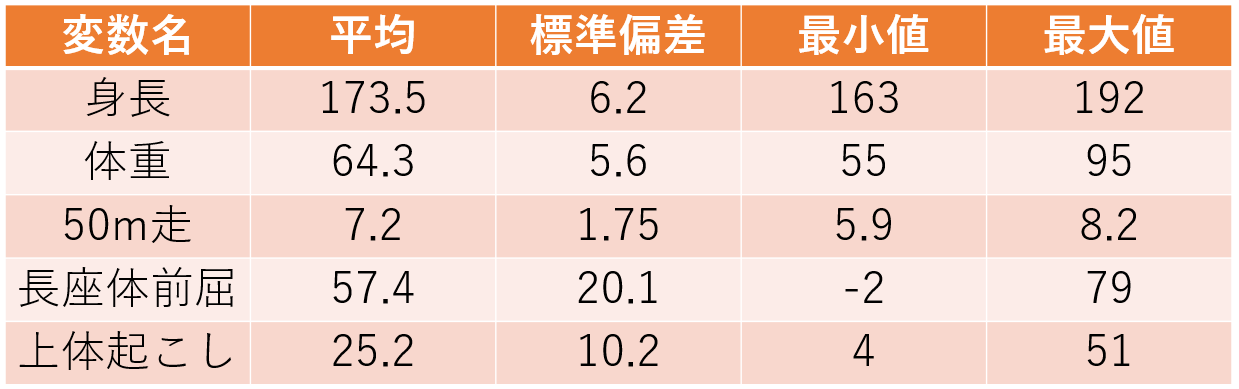
\includegraphics[width=0.8\linewidth]{figs/summary_ex} \end{center}

\begin{itemize}
\tightlist
\item
  何らかの介入の効果(法改正や就学、ナッジによる行動変容など\ldots)を検証したい場合は、介入群と統制群が似た集団であることを確認するため、両者を分けて要約統計量を作成する場合も
\item
  様々な関数を利用できるので、目的に応じて好きなものを使う
\end{itemize}
\end{block}

\begin{block}{ペンギンデータの要約統計量}
\protect\hypertarget{ux30daux30f3ux30aeux30f3ux30c7ux30fcux30bfux306eux8981ux7d04ux7d71ux8a08ux91cf}{}
\begin{itemize}
\tightlist
\item
  最もシンプルなのはsummary関数

  \begin{itemize}
  \tightlist
  \item
    各変数の主要な統計量を記載してくれる
  \end{itemize}
\end{itemize}

\begin{Shaded}
\begin{Highlighting}[]
\NormalTok{palmerpenguins}\SpecialCharTok{::}\NormalTok{penguins }\SpecialCharTok{\%\textgreater{}\%}
  \FunctionTok{summary}\NormalTok{()}
\end{Highlighting}
\end{Shaded}

\begin{verbatim}
##       species          island    bill_length_mm  bill_depth_mm  
##  Adelie   :152   Biscoe   :168   Min.   :32.10   Min.   :13.10  
##  Chinstrap: 68   Dream    :124   1st Qu.:39.23   1st Qu.:15.60  
##  Gentoo   :124   Torgersen: 52   Median :44.45   Median :17.30  
##                                  Mean   :43.92   Mean   :17.15  
##                                  3rd Qu.:48.50   3rd Qu.:18.70  
##                                  Max.   :59.60   Max.   :21.50  
##                                  NA's   :2       NA's   :2      
##  flipper_length_mm  body_mass_g       sex           year     
##  Min.   :172.0     Min.   :2700   female:165   Min.   :2007  
##  1st Qu.:190.0     1st Qu.:3550   male  :168   1st Qu.:2007  
##  Median :197.0     Median :4050   NA's  : 11   Median :2008  
##  Mean   :200.9     Mean   :4202                Mean   :2008  
##  3rd Qu.:213.0     3rd Qu.:4750                3rd Qu.:2009  
##  Max.   :231.0     Max.   :6300                Max.   :2009  
##  NA's   :2         NA's   :2
\end{verbatim}
\end{block}

\begin{block}{データを整理する}
\protect\hypertarget{ux30c7ux30fcux30bfux3092ux6574ux7406ux3059ux308b}{}
\begin{itemize}
\tightlist
\item
  取得したデータはそのまま分析に使えるわけではない

  \begin{itemize}
  \tightlist
  \item
    必要な情報が抜け落ちている場合や、アンケートの設問の誤解等で明らかにおかしな回答が存在することがある
  \item
    情報が全て入っているが、その分析に関しては不適当な観測が含まれる場合も
  \item
    分析の対象でない観測が一緒に含まれている場合(例えば男性労働者の行動に注目したいときに、女性労働者を含めたまま分析を行うのは不適当)
  \item
    元データの情報を用いて、新たに変数を作りたい場合もある(例えば、5段階で回答された幸福度を1,2と3-5の2つに再分類した変数を作成する)
  \end{itemize}
\item
  これらの問題を解決し、分析に利用可能なデータセットを作成することを「データの整理」「データクリーニング」と呼ぶ
\item
  tidyverseパッケージから、便利な関数がたくさん提供されている

  \begin{itemize}
  \tightlist
  \item
    \texttt{filter}関数:行を絞る
  \item
    \texttt{select}関数:列を絞る
  \item
    \texttt{mutate}関数:新しい変数を作成する
  \item
    \texttt{split}関数:データフレームをリストに分割する
  \end{itemize}
\end{itemize}
\end{block}

\begin{block}{列名の付け直し}
\protect\hypertarget{ux5217ux540dux306eux4ed8ux3051ux76f4ux3057}{}
\begin{itemize}
\tightlist
\item
  列名は原則アルファベットとアンダースコア(\_)で付けておく方がエラーが起こりにくい

  \begin{itemize}
  \tightlist
  \item
    日本語がギリセーフ、アンダースコア以外の記号や引用符は使わない
  \item
    数字は2文字目以降にしか使えない
  \end{itemize}
\item
  もし入っている場合は、\texttt{rename} 関数もしくは\texttt{set\_names}
  関数を用いて列名を変更した方が良い
\end{itemize}

\begin{Shaded}
\begin{Highlighting}[]
\NormalTok{palmerpenguins}\SpecialCharTok{::}\NormalTok{penguins }\SpecialCharTok{\%\textgreater{}\%}
\NormalTok{  dplyr}\SpecialCharTok{::}\FunctionTok{rename}\NormalTok{(}\AttributeTok{weight =}\NormalTok{ body\_mass\_g) }\SpecialCharTok{\%\textgreater{}\%} \CommentTok{\# body\_mass\_g を weightに}
  \FunctionTok{head}\NormalTok{(}\DecValTok{2}\NormalTok{)}
\end{Highlighting}
\end{Shaded}

\begin{verbatim}
## # A tibble: 2 x 8
##   species island    bill_length_mm bill_depth_mm flipper_length_mm weight sex   
##   <fct>   <fct>              <dbl>         <dbl>             <int>  <int> <fct> 
## 1 Adelie  Torgersen           39.1          18.7               181   3750 male  
## 2 Adelie  Torgersen           39.5          17.4               186   3800 female
## # ... with 1 more variable: year <int>
\end{verbatim}
\end{block}

\begin{block}{列名の付け直し (cont'd)}
\protect\hypertarget{ux5217ux540dux306eux4ed8ux3051ux76f4ux3057-contd}{}
\begin{itemize}
\tightlist
\item
  \texttt{set\_names}
  はそのデータセットの列名をまとめて変更する:列数と同じ長さのchr型ベクトルを指定
\end{itemize}

\begin{Shaded}
\begin{Highlighting}[]
\NormalTok{newnames }\OtherTok{\textless{}{-}} \FunctionTok{c}\NormalTok{(}\StringTok{"species"}\NormalTok{, }\StringTok{"island"}\NormalTok{, }\StringTok{"bill\_lg"}\NormalTok{, }\StringTok{"bill\_dep"}\NormalTok{, }\StringTok{"flipper"}\NormalTok{, }\StringTok{"weight"}\NormalTok{, }\StringTok{"sex"}\NormalTok{, }\StringTok{"yr"}\NormalTok{)}
\NormalTok{palmerpenguins}\SpecialCharTok{::}\NormalTok{penguins }\SpecialCharTok{\%\textgreater{}\%}
\NormalTok{  purrr}\SpecialCharTok{::}\FunctionTok{set\_names}\NormalTok{(newnames) }\SpecialCharTok{\%\textgreater{}\%}
  \FunctionTok{head}\NormalTok{(}\DecValTok{2}\NormalTok{) }\SpecialCharTok{\%\textgreater{}\%}
  \FunctionTok{print}\NormalTok{()}
\end{Highlighting}
\end{Shaded}

\begin{verbatim}
## # A tibble: 2 x 8
##   species island    bill_lg bill_dep flipper weight sex       yr
##   <fct>   <fct>       <dbl>    <dbl>   <int>  <int> <fct>  <int>
## 1 Adelie  Torgersen    39.1     18.7     181   3750 male    2007
## 2 Adelie  Torgersen    39.5     17.4     186   3800 female  2007
\end{verbatim}
\end{block}

\begin{block}{データを絞る}
\protect\hypertarget{ux30c7ux30fcux30bfux3092ux7d5eux308b}{}
\begin{itemize}
\tightlist
\item
  条件にあてはまる行を抜き出す:filter関数を利用
\item
  条件式の書き方

  \begin{itemize}
  \tightlist
  \item
    参照する列を記述し、「〇〇に一致する場合」「〇〇より大きい/小さい場合」などの条件をRのルールに従って記述する

    \begin{itemize}
    \tightlist
    \item
      \texttt{A\ ==\ B}: A列の内容がBと完全に一致,
      Bが文字列の場合はクオーテーションで囲う
    \item
      \texttt{A\ \textgreater{}=\ B}: B以上の値,
      逆なら\texttt{\textless{}=}
    \item
      \texttt{A\ \%in\%\ c(B,\ C,\ D)}: A列の要素がベクトルの要素B, C,
      Dのいずれかに一致
    \item
      否定は!: \texttt{A\ !=\ B}, \texttt{!(A\ \%in\%\ c(a,\ b,\ c))}
    \end{itemize}
  \item
    and条件は\&, or条件は\textbar で繋ぐ:条件1 \textbar{} 条件2
    なら、1,2いずれかの条件にあてはまるもの
  \end{itemize}
\end{itemize}

\begin{Shaded}
\begin{Highlighting}[]
\NormalTok{df }\OtherTok{\textless{}{-}}\NormalTok{ palmerpenguins}\SpecialCharTok{::}\NormalTok{penguins }\SpecialCharTok{\%\textgreater{}\%}
\NormalTok{  dplyr}\SpecialCharTok{::}\FunctionTok{filter}\NormalTok{(species }\SpecialCharTok{==} \StringTok{"Gentoo"}\NormalTok{) }\CommentTok{\# ジェンツーペンギンのみに絞る}

\FunctionTok{print}\NormalTok{(df }\SpecialCharTok{\%\textgreater{}\%} \FunctionTok{head}\NormalTok{(}\DecValTok{2}\NormalTok{))}
\end{Highlighting}
\end{Shaded}

\begin{verbatim}
## # A tibble: 2 x 8
##   species island bill_length_mm bill_depth_mm flipper_length_~ body_mass_g sex  
##   <fct>   <fct>           <dbl>         <dbl>            <int>       <int> <fct>
## 1 Gentoo  Biscoe           46.1          13.2              211        4500 fema~
## 2 Gentoo  Biscoe           50            16.3              230        5700 male 
## # ... with 1 more variable: year <int>
\end{verbatim}
\end{block}

\begin{block}{欠損値}
\protect\hypertarget{ux6b20ux640dux5024}{}
\begin{itemize}
\tightlist
\item
  欠損値(分からない、無回答などの理由で値が入っていない)がある場合、そのセルを取り除いて分析を行うことがある
\item
  Rでは、\texttt{NA}で表す:型は勝手に判断してくれる場合と、してくれない場合とがある

  \begin{itemize}
  \tightlist
  \item
    \texttt{NA\_real\_}: num型
  \item
    \texttt{NA\_character}: chr型
  \end{itemize}
\item
  「欠損である」という条件を表す関数:\texttt{is.na()}

  \begin{itemize}
  \tightlist
  \item
    括弧内の値が欠損であるかどうかを返す: filterなどの条件に指定
  \end{itemize}
\end{itemize}

\begin{Shaded}
\begin{Highlighting}[]
\NormalTok{palmerpenguins}\SpecialCharTok{::}\NormalTok{penguins }\SpecialCharTok{\%\textgreater{}\%} \FunctionTok{nrow}\NormalTok{() }\CommentTok{\# 列数を返す}
\end{Highlighting}
\end{Shaded}

\begin{verbatim}
## [1] 344
\end{verbatim}

\begin{Shaded}
\begin{Highlighting}[]
\NormalTok{palmerpenguins}\SpecialCharTok{::}\NormalTok{penguins }\SpecialCharTok{\%\textgreater{}\%}
  \FunctionTok{filter}\NormalTok{(}\SpecialCharTok{!}\FunctionTok{is.na}\NormalTok{(body\_mass\_g)) }\SpecialCharTok{\%\textgreater{}\%} \CommentTok{\# 体重が欠損している個体を除外}
  \FunctionTok{nrow}\NormalTok{() }\CommentTok{\#上より列数が減っている}
\end{Highlighting}
\end{Shaded}

\begin{verbatim}
## [1] 342
\end{verbatim}
\end{block}

\begin{block}{情報を絞る}
\protect\hypertarget{ux60c5ux5831ux3092ux7d5eux308b}{}
\begin{itemize}
\tightlist
\item
  全ての列を必要としない場合:select関数を利用
\item
  残したい列を順番に列挙するだけでOK。列番号でもよい
\item
  落としたい列を-(マイナス)で指定してもよい
\end{itemize}

\begin{Shaded}
\begin{Highlighting}[]
\NormalTok{df }\OtherTok{\textless{}{-}}\NormalTok{ palmerpenguins}\SpecialCharTok{::}\NormalTok{penguins }\SpecialCharTok{\%\textgreater{}\%}
\NormalTok{  dplyr}\SpecialCharTok{::}\FunctionTok{select}\NormalTok{(species, sex, }\DecValTok{5}\NormalTok{, }\DecValTok{6}\NormalTok{)}

\FunctionTok{print}\NormalTok{(df }\SpecialCharTok{\%\textgreater{}\%} \FunctionTok{head}\NormalTok{(}\DecValTok{4}\NormalTok{))}
\end{Highlighting}
\end{Shaded}

\begin{verbatim}
## # A tibble: 4 x 4
##   species sex    flipper_length_mm body_mass_g
##   <fct>   <fct>              <int>       <int>
## 1 Adelie  male                 181        3750
## 2 Adelie  female               186        3800
## 3 Adelie  female               195        3250
## 4 Adelie  <NA>                  NA          NA
\end{verbatim}

\begin{itemize}
\tightlist
\item
  取り出した列をベクトルとして利用したい場合:\texttt{pull}関数で抜き出し可能
\end{itemize}
\end{block}

\begin{block}{新しい変数を作成する}
\protect\hypertarget{ux65b0ux3057ux3044ux5909ux6570ux3092ux4f5cux6210ux3059ux308b}{}
\begin{itemize}
\tightlist
\item
  今ある情報を元に、新しい列を作成することがある:\texttt{mutate}関数を利用する

  \begin{itemize}
  \tightlist
  \item
    列の変数型が数値の場合: 四則演算の演算子をそのまま利用できる
  \item
    特定の条件にあてはまるか否かを判定して数値を代入したい場合:\texttt{if\_else}関数、\texttt{case\_when}関数を利用
  \end{itemize}
\end{itemize}

\begin{Shaded}
\begin{Highlighting}[]
\NormalTok{df }\OtherTok{\textless{}{-}}\NormalTok{ palmerpenguins}\SpecialCharTok{::}\NormalTok{penguins }\SpecialCharTok{\%\textgreater{}\%}
  \FunctionTok{mutate}\NormalTok{(}
    \AttributeTok{flipper\_length\_2 =}\NormalTok{ flipper\_length\_mm}\SpecialCharTok{\^{}}\DecValTok{2}\NormalTok{, }\CommentTok{\# 羽根の長さの2乗}
    \AttributeTok{weight\_size =} \FunctionTok{if\_else}\NormalTok{(}\AttributeTok{condition =}\NormalTok{ body\_mass\_g }\SpecialCharTok{\textgreater{}=} \DecValTok{4050}\NormalTok{, }\AttributeTok{true =} \StringTok{"L"}\NormalTok{, }\AttributeTok{false =} \StringTok{"F"}\NormalTok{),}
    \AttributeTok{flipper\_size\_3 =} \FunctionTok{case\_when}\NormalTok{(}
\NormalTok{      body\_mass\_g }\SpecialCharTok{\textless{}=} \DecValTok{3550} \SpecialCharTok{\textasciitilde{}} \StringTok{"S"}\NormalTok{,}
\NormalTok{      body\_mass\_g }\SpecialCharTok{\textgreater{}=} \DecValTok{3550} \SpecialCharTok{\&}\NormalTok{ body\_mass\_g }\SpecialCharTok{\textless{}=} \DecValTok{4750} \SpecialCharTok{\textasciitilde{}} \StringTok{"M"}\NormalTok{,}
      \ConstantTok{TRUE} \SpecialCharTok{\textasciitilde{}} \StringTok{"L"} \CommentTok{\# TRUE はそれ以外}
\NormalTok{    )}
\NormalTok{  )}
\end{Highlighting}
\end{Shaded}
\end{block}

\begin{block}{作成した変数を確認}
\protect\hypertarget{ux4f5cux6210ux3057ux305fux5909ux6570ux3092ux78baux8a8d}{}
\begin{verbatim}
## # A tibble: 344 x 6
##    species island    body_mass_g flipper_length_2 weight_size flipper_size_3
##    <fct>   <fct>           <int>            <dbl> <chr>       <chr>         
##  1 Adelie  Torgersen        3750            32761 F           M             
##  2 Adelie  Torgersen        3800            34596 F           M             
##  3 Adelie  Torgersen        3250            38025 F           S             
##  4 Adelie  Torgersen          NA               NA <NA>        L             
##  5 Adelie  Torgersen        3450            37249 F           S             
##  6 Adelie  Torgersen        3650            36100 F           M             
##  7 Adelie  Torgersen        3625            32761 F           M             
##  8 Adelie  Torgersen        4675            38025 L           M             
##  9 Adelie  Torgersen        3475            37249 F           S             
## 10 Adelie  Torgersen        4250            36100 L           M             
## # ... with 334 more rows
\end{verbatim}
\end{block}

\begin{block}{サンプルを分割する}
\protect\hypertarget{ux30b5ux30f3ux30d7ux30ebux3092ux5206ux5272ux3059ux308b}{}
\begin{itemize}
\tightlist
\item
  サンプルを特定の変数の値ごとに分割したい時がある

  \begin{itemize}
  \tightlist
  \item
    例えば、オスのサンプルとメスのサンプルを分割する
  \item
    \texttt{filter}関数を使ってもいいが、例えば雄雌それぞれのサンプルに同じ操作を適用したい場合などは、コードが冗長になる場合がある
  \item
    \texttt{split}関数と\texttt{pull}関数を組み合わせて使うと、データフレームをリスト形式で分割できる
  \end{itemize}
\end{itemize}

\begin{Shaded}
\begin{Highlighting}[]
\NormalTok{df\_split }\OtherTok{\textless{}{-}}\NormalTok{ palmerpenguins}\SpecialCharTok{::}\NormalTok{penguins }\SpecialCharTok{\%\textgreater{}\%}
  \FunctionTok{select}\NormalTok{(species, island, sex) }\SpecialCharTok{\%\textgreater{}\%} \CommentTok{\# 表示の都合上列数を限定}
  \FunctionTok{split}\NormalTok{(}\FunctionTok{pull}\NormalTok{(., sex)) }\CommentTok{\# 分割の基準にしたい変数を入力}
\FunctionTok{print}\NormalTok{(df\_split)}
\end{Highlighting}
\end{Shaded}

\begin{verbatim}
## $female
## # A tibble: 165 x 3
##    species island    sex   
##    <fct>   <fct>     <fct> 
##  1 Adelie  Torgersen female
##  2 Adelie  Torgersen female
##  3 Adelie  Torgersen female
##  4 Adelie  Torgersen female
##  5 Adelie  Torgersen female
##  6 Adelie  Torgersen female
##  7 Adelie  Torgersen female
##  8 Adelie  Torgersen female
##  9 Adelie  Biscoe    female
## 10 Adelie  Biscoe    female
## # ... with 155 more rows
## 
## $male
## # A tibble: 168 x 3
##    species island    sex  
##    <fct>   <fct>     <fct>
##  1 Adelie  Torgersen male 
##  2 Adelie  Torgersen male 
##  3 Adelie  Torgersen male 
##  4 Adelie  Torgersen male 
##  5 Adelie  Torgersen male 
##  6 Adelie  Torgersen male 
##  7 Adelie  Torgersen male 
##  8 Adelie  Biscoe    male 
##  9 Adelie  Biscoe    male 
## 10 Adelie  Biscoe    male 
## # ... with 158 more rows
\end{verbatim}
\end{block}

\begin{block}{その他データ操作関連の関数}
\protect\hypertarget{ux305dux306eux4ed6ux30c7ux30fcux30bfux64cdux4f5cux95a2ux9023ux306eux95a2ux6570}{}
\begin{itemize}
\tightlist
\item
  stringr, stringi パッケージは文字列の処理に便利

  \begin{itemize}
  \tightlist
  \item
    先頭から何文字、指定した条件に合致した文字を抜き出しなど、character型の文字列を操作するのに非常に便利
  \end{itemize}
\end{itemize}
\end{block}

\begin{block}{もっと便利な要約統計量}
\protect\hypertarget{ux3082ux3063ux3068ux4fbfux5229ux306aux8981ux7d04ux7d71ux8a08ux91cf}{}
\end{block}

\begin{block}{dplyr パッケージの利用}
\protect\hypertarget{dplyr-ux30d1ux30c3ux30b1ux30fcux30b8ux306eux5229ux7528}{}
\begin{itemize}
\tightlist
\item
  dplyr: tidyverseパッケージに含まれるデータ操作系の関数の一つ
\item
  \texttt{group\_by}
  関数は、以降の操作を指定した変数ごとに行うことを宣言する関数

  \begin{itemize}
  \tightlist
  \item
    例えば、\texttt{group\_by(species)}とすると、以降の操作はペンギンの種類ごとに行われる
  \end{itemize}
\item
  \texttt{summarise}
  関数は、データフレームの指定された列を任意の関数で集計するための関数
\end{itemize}

\begin{Shaded}
\begin{Highlighting}[]
\NormalTok{palmerpenguins}\SpecialCharTok{::}\NormalTok{penguins }\SpecialCharTok{\%\textgreater{}\%}
  \FunctionTok{summarise}\NormalTok{(}
    \AttributeTok{mean\_bill\_length\_mm =} \FunctionTok{mean}\NormalTok{(bill\_length\_mm, }\AttributeTok{na.rm =}\NormalTok{ T), }\CommentTok{\# くちばしの長さの平均を取る、欠損値は除外}
    \AttributeTok{mean\_flipper\_length\_mm =} \FunctionTok{mean}\NormalTok{(flipper\_length\_mm, }\AttributeTok{na.rm =}\NormalTok{ T),}
    \AttributeTok{mean\_body\_mass\_g =} \FunctionTok{mean}\NormalTok{(body\_mass\_g, }\AttributeTok{na.rm =}\NormalTok{ T),}
\NormalTok{  )}
\end{Highlighting}
\end{Shaded}

\begin{verbatim}
## # A tibble: 1 x 3
##   mean_bill_length_mm mean_flipper_length_mm mean_body_mass_g
##                 <dbl>                  <dbl>            <dbl>
## 1                43.9                   201.            4202.
\end{verbatim}

\begin{itemize}
\tightlist
\item
  任意の統計量、変数を自由に選択肢して表を作ることができる
\end{itemize}
\end{block}

\begin{block}{group\_byを組み合わせる}
\protect\hypertarget{group_byux3092ux7d44ux307fux5408ux308fux305bux308b}{}
\begin{Shaded}
\begin{Highlighting}[]
\NormalTok{palmerpenguins}\SpecialCharTok{::}\NormalTok{penguins }\SpecialCharTok{\%\textgreater{}\%}
  \FunctionTok{group\_by}\NormalTok{(species) }\SpecialCharTok{\%\textgreater{}\%} \CommentTok{\# 種類ごとに}
  \FunctionTok{summarise}\NormalTok{(}
    \AttributeTok{N =} \FunctionTok{n}\NormalTok{(), }\CommentTok{\# サンプルサイズ}
    \AttributeTok{mean\_bill\_length\_mm =} \FunctionTok{mean}\NormalTok{(bill\_length\_mm, }\AttributeTok{na.rm =}\NormalTok{ T), }\CommentTok{\# くちばしの長さの平均を取る、欠損値は除外}
    \AttributeTok{mean\_flipper\_length\_mm =} \FunctionTok{mean}\NormalTok{(flipper\_length\_mm, }\AttributeTok{na.rm =}\NormalTok{ T),}
    \AttributeTok{mean\_body\_mass\_g =} \FunctionTok{mean}\NormalTok{(body\_mass\_g, }\AttributeTok{na.rm =}\NormalTok{ T),}
\NormalTok{  )}
\end{Highlighting}
\end{Shaded}

\begin{verbatim}
## # A tibble: 3 x 5
##   species       N mean_bill_length_mm mean_flipper_length_mm mean_body_mass_g
##   <fct>     <int>               <dbl>                  <dbl>            <dbl>
## 1 Adelie      152                38.8                   190.            3701.
## 2 Chinstrap    68                48.8                   196.            3733.
## 3 Gentoo      124                47.5                   217.            5076.
\end{verbatim}

\begin{itemize}
\tightlist
\item
  ペンギンの種類間での平均の比較が可能に
\end{itemize}
\end{block}

\begin{block}{group\_byを組み合わせる}
\protect\hypertarget{group_byux3092ux7d44ux307fux5408ux308fux305bux308b-1}{}
\begin{itemize}
\tightlist
\item
  複数変数を指定してもOK
\end{itemize}

\begin{Shaded}
\begin{Highlighting}[]
\NormalTok{palmerpenguins}\SpecialCharTok{::}\NormalTok{penguins }\SpecialCharTok{\%\textgreater{}\%}
  \FunctionTok{group\_by}\NormalTok{(sex, species) }\SpecialCharTok{\%\textgreater{}\%} \CommentTok{\# 種類と性別ごとに}
  \FunctionTok{summarise}\NormalTok{(}
    \AttributeTok{N =} \FunctionTok{n}\NormalTok{(),}
    \AttributeTok{mean\_bill\_length\_mm =} \FunctionTok{mean}\NormalTok{(bill\_length\_mm, }\AttributeTok{na.rm =}\NormalTok{ T), }\CommentTok{\# くちばしの長さの平均を取る、欠損値は除外}
    \AttributeTok{mean\_flipper\_length\_mm =} \FunctionTok{mean}\NormalTok{(flipper\_length\_mm, }\AttributeTok{na.rm =}\NormalTok{ T),}
    \AttributeTok{mean\_body\_mass\_g =} \FunctionTok{mean}\NormalTok{(body\_mass\_g, }\AttributeTok{na.rm =}\NormalTok{ T),}
\NormalTok{  )}
\end{Highlighting}
\end{Shaded}

\begin{verbatim}
## `summarise()` has grouped output by 'sex'. You can override using the `.groups`
## argument.
\end{verbatim}

\begin{verbatim}
## # A tibble: 8 x 6
## # Groups:   sex [3]
##   sex    species       N mean_bill_length_mm mean_flipper_leng~ mean_body_mass_g
##   <fct>  <fct>     <int>               <dbl>              <dbl>            <dbl>
## 1 female Adelie       73                37.3               188.            3369.
## 2 female Chinstrap    34                46.6               192.            3527.
## 3 female Gentoo       58                45.6               213.            4680.
## 4 male   Adelie       73                40.4               192.            4043.
## 5 male   Chinstrap    34                51.1               200.            3939.
## 6 male   Gentoo       61                49.5               222.            5485.
## 7 <NA>   Adelie        6                37.8               186.            3540 
## 8 <NA>   Gentoo        5                45.6               216.            4588.
\end{verbatim}

\begin{itemize}
\tightlist
\item
  同様に、標準偏差などを掲載すると良い
\end{itemize}
\end{block}

\begin{block}{skimrパッケージの利用}
\protect\hypertarget{skimrux30d1ux30c3ux30b1ux30fcux30b8ux306eux5229ux7528}{}
\begin{itemize}
\tightlist
\item
  skim関数は各行にデータセットのカラム(列)、各列に統計量を記載した扱いやすい記述統計量を作成してくれる
\end{itemize}

\begin{Shaded}
\begin{Highlighting}[]
\FunctionTok{library}\NormalTok{(skimr)}
\NormalTok{descriptive }\OtherTok{\textless{}{-}}\NormalTok{ palmerpenguins}\SpecialCharTok{::}\NormalTok{penguins }\SpecialCharTok{\%\textgreater{}\%}
  \FunctionTok{skim}\NormalTok{()}
\FunctionTok{print}\NormalTok{(descriptive)}
\end{Highlighting}
\end{Shaded}

\begin{verbatim}
## -- Data Summary ------------------------
##                            Values    
## Name                       Piped data
## Number of rows             344       
## Number of columns          8         
## _______________________              
## Column type frequency:               
##   factor                   3         
##   numeric                  5         
## ________________________             
## Group variables            None      
## 
## -- Variable type: factor -------------------------------------------------------
## # A tibble: 3 x 6
##   skim_variable n_missing complete_rate ordered n_unique
## * <chr>             <int>         <dbl> <lgl>      <int>
## 1 species               0         1     FALSE          3
## 2 island                0         1     FALSE          3
## 3 sex                  11         0.968 FALSE          2
##   top_counts                 
## * <chr>                      
## 1 Ade: 152, Gen: 124, Chi: 68
## 2 Bis: 168, Dre: 124, Tor: 52
## 3 mal: 168, fem: 165         
## 
## -- Variable type: numeric ------------------------------------------------------
## # A tibble: 5 x 11
##   skim_variable     n_missing complete_rate   mean      sd     p0    p25    p50
## * <chr>                 <int>         <dbl>  <dbl>   <dbl>  <dbl>  <dbl>  <dbl>
## 1 bill_length_mm            2         0.994   43.9   5.46    32.1   39.2   44.4
## 2 bill_depth_mm             2         0.994   17.2   1.97    13.1   15.6   17.3
## 3 flipper_length_mm         2         0.994  201.   14.1    172    190    197  
## 4 body_mass_g               2         0.994 4202.  802.    2700   3550   4050  
## 5 year                      0         1     2008.    0.818 2007   2007   2008  
##      p75   p100 hist 
## *  <dbl>  <dbl> <chr>
## 1   48.5   59.6 <U+2583><U+2587><U+2587><U+2586><U+2581>
## 2   18.7   21.5 <U+2585><U+2585><U+2587><U+2587><U+2582>
## 3  213    231   <U+2582><U+2587><U+2583><U+2585><U+2582>
## 4 4750   6300   <U+2583><U+2587><U+2586><U+2583><U+2582>
## 5 2009   2009   <U+2587><U+2581><U+2587><U+2581><U+2587>
\end{verbatim}
\end{block}

\begin{block}{質的変数と量的変数}
\protect\hypertarget{ux8ceaux7684ux5909ux6570ux3068ux91cfux7684ux5909ux6570}{}
\begin{itemize}
\tightlist
\item
  \texttt{yank}関数:skimで要約した列のうち、特定の型を持つ値の要約のみを抜き出して記載する関数
\end{itemize}

\begin{Shaded}
\begin{Highlighting}[]
\NormalTok{palmerpenguins}\SpecialCharTok{::}\NormalTok{penguins }\SpecialCharTok{\%\textgreater{}\%}
  \FunctionTok{skim}\NormalTok{() }\SpecialCharTok{\%\textgreater{}\%}
  \FunctionTok{yank}\NormalTok{(., }\AttributeTok{skim\_type =} \StringTok{"numeric"}\NormalTok{) }\SpecialCharTok{\%\textgreater{}\%} \CommentTok{\# numeric型の要約統計量を表示}
  \FunctionTok{print}\NormalTok{()}
\end{Highlighting}
\end{Shaded}

\begin{verbatim}
## 
## -- Variable type: numeric ------------------------------------------------------
## # A tibble: 5 x 11
##   skim_variable     n_missing complete_rate   mean      sd     p0    p25    p50
## * <chr>                 <int>         <dbl>  <dbl>   <dbl>  <dbl>  <dbl>  <dbl>
## 1 bill_length_mm            2         0.994   43.9   5.46    32.1   39.2   44.4
## 2 bill_depth_mm             2         0.994   17.2   1.97    13.1   15.6   17.3
## 3 flipper_length_mm         2         0.994  201.   14.1    172    190    197  
## 4 body_mass_g               2         0.994 4202.  802.    2700   3550   4050  
## 5 year                      0         1     2008.    0.818 2007   2007   2008  
##      p75   p100 hist 
## *  <dbl>  <dbl> <chr>
## 1   48.5   59.6 <U+2583><U+2587><U+2587><U+2586><U+2581>
## 2   18.7   21.5 <U+2585><U+2585><U+2587><U+2587><U+2582>
## 3  213    231   <U+2582><U+2587><U+2583><U+2585><U+2582>
## 4 4750   6300   <U+2583><U+2587><U+2586><U+2583><U+2582>
## 5 2009   2009   <U+2587><U+2581><U+2587><U+2581><U+2587>
\end{verbatim}
\end{block}

\begin{block}{グループごとの統計量}
\protect\hypertarget{ux30b0ux30ebux30fcux30d7ux3054ux3068ux306eux7d71ux8a08ux91cf}{}
\begin{itemize}
\tightlist
\item
  skimにもgroup\_by関数を適用可能
\end{itemize}

\begin{Shaded}
\begin{Highlighting}[]
\NormalTok{sum }\OtherTok{\textless{}{-}}\NormalTok{ palmerpenguins}\SpecialCharTok{::}\NormalTok{penguins }\SpecialCharTok{\%\textgreater{}\%}
  \FunctionTok{group\_by}\NormalTok{(island) }\SpecialCharTok{\%\textgreater{}\%}
  \FunctionTok{skim}\NormalTok{() }\SpecialCharTok{\%\textgreater{}\%}
  \FunctionTok{yank}\NormalTok{(., }\AttributeTok{skim\_type =} \StringTok{"numeric"}\NormalTok{)}

\NormalTok{sum }\SpecialCharTok{\%\textgreater{}\%}
  \FunctionTok{filter}\NormalTok{(skim\_variable }\SpecialCharTok{==} \StringTok{"bill\_length\_mm"}\NormalTok{) }\SpecialCharTok{\%\textgreater{}\%}
  \FunctionTok{filter}\NormalTok{(island }\SpecialCharTok{\%in\%} \FunctionTok{c}\NormalTok{(}\StringTok{\textquotesingle{}Biscoe\textquotesingle{}}\NormalTok{, }\StringTok{\textquotesingle{}Dream\textquotesingle{}}\NormalTok{)) }\SpecialCharTok{\%\textgreater{}\%}
  \FunctionTok{select}\NormalTok{(skim\_variable, island, complete\_rate, mean, sd) }\CommentTok{\# selectで必要な統計量だけ出す}
\end{Highlighting}
\end{Shaded}

\textbf{Variable type: numeric}

\begin{longtable}[]{@{}llrrr@{}}
\toprule
skim\_variable & island & complete\_rate & mean & sd \\
\midrule
\endhead
bill\_length\_mm & Biscoe & 0.99 & 45.26 & 4.77 \\
bill\_length\_mm & Dream & 1.00 & 44.17 & 5.95 \\
\bottomrule
\end{longtable}
\end{block}
\end{frame}

\begin{frame}[fragile]{データの概観:可視化}
\protect\hypertarget{ux30c7ux30fcux30bfux306eux6982ux89b3ux53efux8996ux5316}{}
\begin{itemize}
\tightlist
\item
  データを可視化する:ggplot2パッケージの利用
\item
  ggplotの記法を覚える

  \begin{itemize}
  \tightlist
  \item
    ヒストグラム
  \item
    散布図
  \item
    棒グラフ
  \end{itemize}
\end{itemize}

\begin{block}{データを可視化する}
\protect\hypertarget{ux30c7ux30fcux30bfux3092ux53efux8996ux5316ux3059ux308b}{}
\begin{itemize}
\tightlist
\item
  前章では要約統計量を作成することでデータの概観を把握する方法を学習
\item
  しかし、変数の分布や二変数間の相関、時系列での数値の変化など、要約統計量だけでは捉えきれない性質も存在
\item
  データをグラフの形で可視化することで、分かりやすい・伝わりやすい数値化が可能
\item
  デフォルトで使用できるgraphicsパッケージは早くて便利だが、ggplot2パッケージならより詳細\&手軽な操作で美しいグラフを描画できる
\end{itemize}

\begin{center}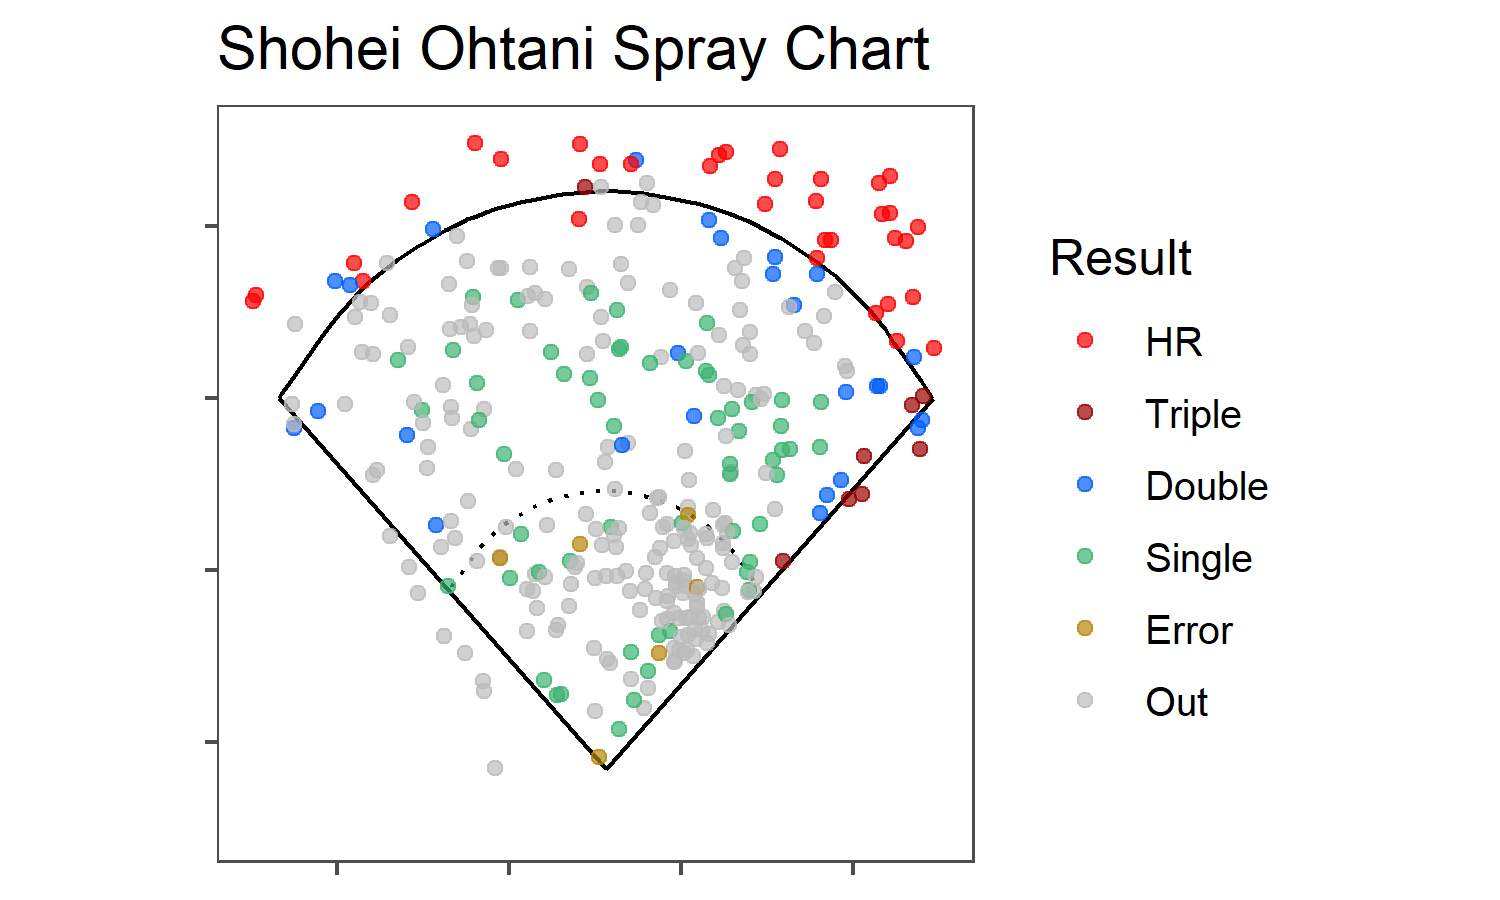
\includegraphics[width=0.5\linewidth]{figs/Ohtani_spray_total} \end{center}
\end{block}

\begin{block}{ggplotの記法}
\protect\hypertarget{ggplotux306eux8a18ux6cd5}{}
\begin{itemize}
\tightlist
\item
  ggplot2パッケージの関数はやや特殊:たくさんの関数を「足し算」することでグラフに手を加えていく
\item
  \texttt{ggplot}
  関数で台紙を作る:どのデータフレームを使って可視化するのかもここで宣言
\end{itemize}

\begin{Shaded}
\begin{Highlighting}[]
\NormalTok{df }\OtherTok{\textless{}{-}}\NormalTok{ palmerpenguins}\SpecialCharTok{::}\NormalTok{penguins}
\NormalTok{ggplot2}\SpecialCharTok{::}\FunctionTok{ggplot}\NormalTok{(}\AttributeTok{data =}\NormalTok{ df) }\CommentTok{\# この時点では白紙}
\end{Highlighting}
\end{Shaded}

\begin{center}\includegraphics[width=0.4\linewidth]{introduction1_files/figure-beamer/unnamed-chunk-56-1} \end{center}
\end{block}

\begin{block}{ggplotの記法 (cont'd)}
\protect\hypertarget{ggplotux306eux8a18ux6cd5-contd}{}
\begin{center}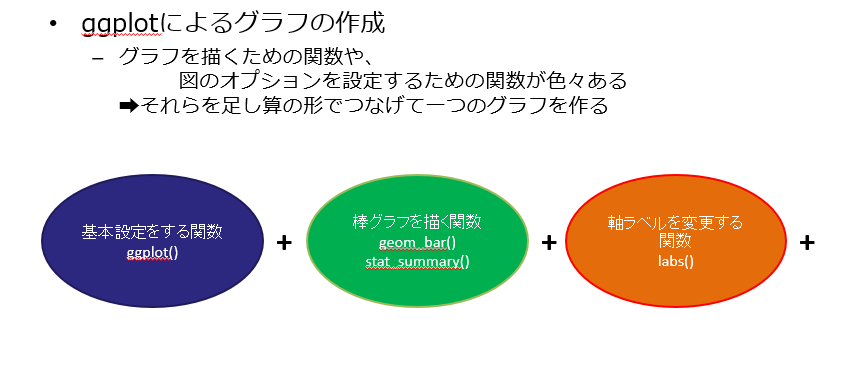
\includegraphics[width=0.8\linewidth]{figs/ggplot_fig} \end{center}
\end{block}

\begin{block}{図形の描画:軸の設定}
\protect\hypertarget{ux56f3ux5f62ux306eux63cfux753bux8ef8ux306eux8a2dux5b9a}{}
\begin{itemize}
\tightlist
\item
  例として、ペンギンの体重のヒストグラムを作ろう:体重という1変数の分布を見る
\item
  \texttt{aes}関数を使い、グラフの横軸・縦軸や色分けの情報を加えていく

  \begin{itemize}
  \tightlist
  \item
    横軸: x, 縦軸: y, グループ分け: group, 色分け: colour, 塗りつぶし:
    shape, 形: shape あたりを覚えておく
  \item
    今回はヒストグラムなので、「横軸が体重ですよ」という情報を渡してやればよい
  \end{itemize}
\item
  その上で、ヒストグラムを描画する関数\texttt{geom\_histogram}関数を加える
\end{itemize}
\end{block}

\begin{block}{ヒストグラムの描画}
\protect\hypertarget{ux30d2ux30b9ux30c8ux30b0ux30e9ux30e0ux306eux63cfux753b}{}
\begin{Shaded}
\begin{Highlighting}[]
\NormalTok{ggplot2}\SpecialCharTok{::}\FunctionTok{ggplot}\NormalTok{(}\AttributeTok{data =}\NormalTok{ df) }\SpecialCharTok{+}
  \FunctionTok{aes}\NormalTok{(}\AttributeTok{x =}\NormalTok{ body\_mass\_g) }\SpecialCharTok{+}
  \FunctionTok{geom\_histogram}\NormalTok{()}
\end{Highlighting}
\end{Shaded}

\begin{verbatim}
## `stat_bin()` using `bins = 30`. Pick better value with `binwidth`.
\end{verbatim}

\begin{verbatim}
## Warning: Removed 2 rows containing non-finite values (stat_bin).
\end{verbatim}

\begin{center}\includegraphics[width=0.5\linewidth]{introduction1_files/figure-beamer/unnamed-chunk-58-1} \end{center}
\end{block}

\begin{block}{細かな体裁の変更}
\protect\hypertarget{ux7d30ux304bux306aux4f53ux88c1ux306eux5909ux66f4}{}
\begin{itemize}
\tightlist
\item
  グラフの背景や軸ラベルを設定する

  \begin{itemize}
  \tightlist
  \item
    背景:\texttt{theme\_〇〇}
    関数で様々な書式を設定できるので、お好みで好きなものを利用。なるべくシンプルなものがよい
  \item
    軸ラベルなど:\texttt{labs}関数で文字を指定、各オプションが対応する場所のテキストが変更される
  \end{itemize}
\end{itemize}

\begin{Shaded}
\begin{Highlighting}[]
\NormalTok{ggplot2}\SpecialCharTok{::}\FunctionTok{ggplot}\NormalTok{(}\AttributeTok{data =}\NormalTok{ df) }\SpecialCharTok{+}
  \FunctionTok{aes}\NormalTok{(}\AttributeTok{x =}\NormalTok{ body\_mass\_g, }\AttributeTok{y =}\NormalTok{ ..density..) }\SpecialCharTok{+}
  \FunctionTok{geom\_histogram}\NormalTok{() }\SpecialCharTok{+}
  \FunctionTok{theme\_bw}\NormalTok{() }\SpecialCharTok{+} \CommentTok{\# 背景の設定}
  \FunctionTok{labs}\NormalTok{(}\AttributeTok{x =} \StringTok{"体重 (g)"}\NormalTok{, }\AttributeTok{y =} \StringTok{"密度"}\NormalTok{, }\AttributeTok{title =} \StringTok{"ぺんぎんの体重分布"}\NormalTok{)}
\end{Highlighting}
\end{Shaded}

\begin{center}\includegraphics[width=0.4\linewidth]{introduction1_files/figure-beamer/unnamed-chunk-59-1} \end{center}
\end{block}

\begin{block}{グループを分けて描画する}
\protect\hypertarget{ux30b0ux30ebux30fcux30d7ux3092ux5206ux3051ux3066ux63cfux753bux3059ux308b}{}
\begin{itemize}
\tightlist
\item
  \texttt{aes}にgroup引数を指定すると、それぞれの描画をグループごとにやってくれる
\item
  同様にcolour・fillを指定すると、グループごとに色分けしてくれる

  \begin{itemize}
  \tightlist
  \item
    通常colour は縁取り、fillは塗りつぶし部分を担当
  \end{itemize}
\end{itemize}

\begin{Shaded}
\begin{Highlighting}[]
\NormalTok{ggplot2}\SpecialCharTok{::}\FunctionTok{ggplot}\NormalTok{(}\AttributeTok{data =}\NormalTok{ df) }\SpecialCharTok{+}
  \FunctionTok{aes}\NormalTok{(}\AttributeTok{x =}\NormalTok{ body\_mass\_g, }\AttributeTok{y =}\NormalTok{ ..density.., }\AttributeTok{group =}\NormalTok{ sex, }\AttributeTok{fill =}\NormalTok{ sex) }\SpecialCharTok{+} 
  \CommentTok{\# 横軸に..density..を指定すると、計数の代わりに密度を出してくれる}
  \FunctionTok{geom\_histogram}\NormalTok{(}\AttributeTok{alpha =}\NormalTok{ .}\DecValTok{5}\NormalTok{) }\SpecialCharTok{+} \CommentTok{\# alpha は透明にするためのオプション}
  \FunctionTok{theme\_bw}\NormalTok{() }\SpecialCharTok{+} \CommentTok{\# 背景の設定}
  \FunctionTok{labs}\NormalTok{(}\AttributeTok{x =} \StringTok{"体重 (g)"}\NormalTok{, }\AttributeTok{y =} \StringTok{"密度"}\NormalTok{, }\AttributeTok{title =} \StringTok{"ぺんぎんの体重分布"}\NormalTok{, }\AttributeTok{fill =} \StringTok{"性別"}\NormalTok{)}
\end{Highlighting}
\end{Shaded}

\begin{center}\includegraphics[width=0.4\linewidth]{introduction1_files/figure-beamer/unnamed-chunk-60-1} \end{center}
\end{block}

\begin{block}{散布図:二変数間の関係を可視化する}
\protect\hypertarget{ux6563ux5e03ux56f3ux4e8cux5909ux6570ux9593ux306eux95a2ux4fc2ux3092ux53efux8996ux5316ux3059ux308b}{}
\begin{itemize}
\tightlist
\item
  散布図は二変数間の関係を示すのに便利:\texttt{geom\_point}関数を利用
\item
  横軸と縦軸両方に変数が必要
\item
\end{itemize}

\begin{Shaded}
\begin{Highlighting}[]
\NormalTok{ggplot2}\SpecialCharTok{::}\FunctionTok{ggplot}\NormalTok{(df) }\SpecialCharTok{+}
\NormalTok{  ggplot2}\SpecialCharTok{::}\FunctionTok{aes}\NormalTok{(}\AttributeTok{x =}\NormalTok{ body\_mass\_g, }\AttributeTok{y =}\NormalTok{ bill\_length\_mm, }\AttributeTok{colour =}\NormalTok{ species) }\SpecialCharTok{+}
\NormalTok{  ggplot2}\SpecialCharTok{::}\FunctionTok{geom\_point}\NormalTok{() }\SpecialCharTok{+}
\NormalTok{  ggplot2}\SpecialCharTok{::}\FunctionTok{geom\_smooth}\NormalTok{(}\AttributeTok{method =} \StringTok{"lm"}\NormalTok{, }\AttributeTok{colour =} \StringTok{"black"}\NormalTok{) }\SpecialCharTok{+} \CommentTok{\# 最小二乗法で近似曲線を描画}
\NormalTok{  ggplot2}\SpecialCharTok{::}\FunctionTok{labs}\NormalTok{(}\AttributeTok{x =} \StringTok{"体重 (g)"}\NormalTok{, }\AttributeTok{y =} \StringTok{"くちばしの長さ (mm)"}\NormalTok{)}
\end{Highlighting}
\end{Shaded}

\begin{center}\includegraphics[width=0.4\linewidth]{introduction1_files/figure-beamer/unnamed-chunk-61-1} \end{center}
\end{block}

\begin{block}{散布図 (cont'd)}
\protect\hypertarget{ux6563ux5e03ux56f3-contd}{}
\begin{Shaded}
\begin{Highlighting}[]
\NormalTok{ggplot2}\SpecialCharTok{::}\FunctionTok{ggplot}\NormalTok{(df) }\SpecialCharTok{+}
\NormalTok{  ggplot2}\SpecialCharTok{::}\FunctionTok{aes}\NormalTok{(}\AttributeTok{x =}\NormalTok{ body\_mass\_g, }\AttributeTok{y =}\NormalTok{ bill\_length\_mm, }\AttributeTok{colour =}\NormalTok{ species, }\AttributeTok{group =}\NormalTok{ species) }\SpecialCharTok{+}
\NormalTok{  ggplot2}\SpecialCharTok{::}\FunctionTok{geom\_point}\NormalTok{() }\SpecialCharTok{+}
\NormalTok{  ggplot2}\SpecialCharTok{::}\FunctionTok{geom\_smooth}\NormalTok{(}\AttributeTok{method =} \StringTok{"lm"}\NormalTok{, }\AttributeTok{colour =} \StringTok{"black"}\NormalTok{) }\SpecialCharTok{+} \CommentTok{\# 最小二乗法で近似曲線を描画}
\NormalTok{  ggplot2}\SpecialCharTok{::}\FunctionTok{labs}\NormalTok{(}\AttributeTok{x =} \StringTok{"体重 (g)"}\NormalTok{, }\AttributeTok{y =} \StringTok{"くちばしの長さ (mm)"}\NormalTok{)}
\end{Highlighting}
\end{Shaded}

\begin{center}\includegraphics[width=0.4\linewidth]{introduction1_files/figure-beamer/unnamed-chunk-62-1} \end{center}

\begin{itemize}
\tightlist
\item
  group化すると種類ごとに近似曲線を引いてくれる
\end{itemize}
\end{block}

\begin{block}{棒グラフ:グループ間の変数の比較}
\protect\hypertarget{ux68d2ux30b0ux30e9ux30d5ux30b0ux30ebux30fcux30d7ux9593ux306eux5909ux6570ux306eux6bd4ux8f03}{}
\begin{itemize}
\tightlist
\item
  棒グラフを描画する関数は\texttt{geom\_bar}関数だが、データフレームから各値の平均を計算してグラフを作成するのはちょっと面倒くさい
\item
  データの平均値を比較したい場合:\texttt{stat\_summary}で、「平均値を」「棒グラフの形で」描画することをオーダーできる
\end{itemize}

\begin{Shaded}
\begin{Highlighting}[]
\NormalTok{df\_clean }\OtherTok{\textless{}{-}}\NormalTok{ df }\SpecialCharTok{\%\textgreater{}\%}
  \FunctionTok{filter}\NormalTok{(}\SpecialCharTok{!}\FunctionTok{is.na}\NormalTok{(sex)) }\CommentTok{\# 性別不明を取り除く}
\NormalTok{ggplot2}\SpecialCharTok{::}\FunctionTok{ggplot}\NormalTok{(df\_clean) }\SpecialCharTok{+}
\NormalTok{  ggplot2}\SpecialCharTok{::}\FunctionTok{aes}\NormalTok{(}\AttributeTok{x =}\NormalTok{ sex, }\AttributeTok{y =}\NormalTok{ body\_mass\_g, }\AttributeTok{fill =}\NormalTok{ sex) }\SpecialCharTok{+}
\NormalTok{  ggplot2}\SpecialCharTok{::}\FunctionTok{stat\_summary}\NormalTok{(}\AttributeTok{geom =} \StringTok{"bar"}\NormalTok{, }\AttributeTok{fun =} \StringTok{"mean"}\NormalTok{) }\SpecialCharTok{+} \CommentTok{\# 棒グラフを、平均を示す形で}
\NormalTok{  ggplot2}\SpecialCharTok{::}\FunctionTok{stat\_summary}\NormalTok{(}\AttributeTok{geom =} \StringTok{"pointrange"}\NormalTok{, }\AttributeTok{fun.data =} \StringTok{"mean\_se"}\NormalTok{) }\SpecialCharTok{+}
\NormalTok{  ggplot2}\SpecialCharTok{::}\FunctionTok{labs}\NormalTok{(}\AttributeTok{x =} \StringTok{""}\NormalTok{, }\AttributeTok{y =} \StringTok{"体重 (mm)"}\NormalTok{)}
\end{Highlighting}
\end{Shaded}

\begin{center}\includegraphics[width=0.4\linewidth]{introduction1_files/figure-beamer/unnamed-chunk-63-1} \end{center}
\end{block}

\begin{block}{折れ線グラフ:}
\protect\hypertarget{ux6298ux308cux7ddaux30b0ux30e9ux30d5}{}
\begin{Shaded}
\begin{Highlighting}[]
\NormalTok{ggplot2}\SpecialCharTok{::}\FunctionTok{ggplot}\NormalTok{(df) }\SpecialCharTok{+}
\NormalTok{  ggplot2}\SpecialCharTok{::}\FunctionTok{aes}\NormalTok{(}\AttributeTok{x =} \FunctionTok{factor}\NormalTok{(year), }\AttributeTok{y =}\NormalTok{ body\_mass\_g, }\AttributeTok{colour =}\NormalTok{ species, }\AttributeTok{group =}\NormalTok{ species) }\SpecialCharTok{+}
\NormalTok{  ggplot2}\SpecialCharTok{::}\FunctionTok{stat\_summary}\NormalTok{(}\AttributeTok{geom =} \StringTok{"point"}\NormalTok{, }\AttributeTok{fun =} \StringTok{"mean"}\NormalTok{) }\SpecialCharTok{+}
\NormalTok{  ggplot2}\SpecialCharTok{::}\FunctionTok{stat\_summary}\NormalTok{(}\AttributeTok{geom =} \StringTok{"line"}\NormalTok{, }\AttributeTok{fun =} \StringTok{"mean"}\NormalTok{) }\SpecialCharTok{+}
\NormalTok{  ggplot2}\SpecialCharTok{::}\FunctionTok{stat\_summary}\NormalTok{(}\AttributeTok{geom =} \StringTok{"pointrange"}\NormalTok{, }\AttributeTok{fun.data =} \StringTok{"mean\_se"}\NormalTok{) }\SpecialCharTok{+}
\NormalTok{  ggplot2}\SpecialCharTok{::}\FunctionTok{theme\_bw}\NormalTok{() }\SpecialCharTok{+}
\NormalTok{  ggplot2}\SpecialCharTok{::}\FunctionTok{labs}\NormalTok{(}\AttributeTok{x =} \StringTok{""}\NormalTok{, }\AttributeTok{y =} \StringTok{"体重 (mm)"}\NormalTok{)}
\end{Highlighting}
\end{Shaded}

\begin{center}\includegraphics[width=0.4\linewidth]{introduction1_files/figure-beamer/unnamed-chunk-64-1} \end{center}
\end{block}

\begin{block}{グラフそのものを系統ごとに分ける}
\protect\hypertarget{ux30b0ux30e9ux30d5ux305dux306eux3082ux306eux3092ux7cfbux7d71ux3054ux3068ux306bux5206ux3051ux308b}{}
\begin{itemize}
\tightlist
\item
  重ねると見づらいから複数に分けたい
\item
  \texttt{facet\_wrap}関数を使うと、サンプルを分割して別々に表示してくれる

  \begin{itemize}
  \tightlist
  \item
    「\textasciitilde{} 変数名」で分割の基準となるサンプル、nrow = ,
    ncol = で出力の並べ方を指定
  \end{itemize}
\end{itemize}

\begin{Shaded}
\begin{Highlighting}[]
\NormalTok{ggplot2}\SpecialCharTok{::}\FunctionTok{ggplot}\NormalTok{(df) }\SpecialCharTok{+}
\NormalTok{  ggplot2}\SpecialCharTok{::}\FunctionTok{aes}\NormalTok{(}\AttributeTok{x =}\NormalTok{ body\_mass\_g, }\AttributeTok{y =}\NormalTok{ bill\_length\_mm, }\AttributeTok{fill =}\NormalTok{ species) }\SpecialCharTok{+}
\NormalTok{  ggplot2}\SpecialCharTok{::}\FunctionTok{geom\_point}\NormalTok{(}\AttributeTok{colour =} \StringTok{"black"}\NormalTok{, }\AttributeTok{shape =} \StringTok{"circle filled"}\NormalTok{) }\SpecialCharTok{+}
\NormalTok{  ggplot2}\SpecialCharTok{::}\FunctionTok{scale\_fill\_viridis\_d}\NormalTok{() }\SpecialCharTok{+} \CommentTok{\# 色分けに関する設定を行う関数:塗る色の指定}
\NormalTok{  ggplot2}\SpecialCharTok{::}\FunctionTok{theme\_bw}\NormalTok{() }\SpecialCharTok{+}
\NormalTok{  ggplot2}\SpecialCharTok{::}\FunctionTok{labs}\NormalTok{(}\AttributeTok{x =} \StringTok{"体重 (g)"}\NormalTok{, }\AttributeTok{y =} \StringTok{"くちばしの長さ (mm)"}\NormalTok{) }\SpecialCharTok{+}
\NormalTok{  ggplot2}\SpecialCharTok{::}\FunctionTok{facet\_wrap}\NormalTok{(}\AttributeTok{facets =} \SpecialCharTok{\textasciitilde{}}\NormalTok{ island, }\AttributeTok{ncol =} \DecValTok{3}\NormalTok{, }\AttributeTok{nrow =} \DecValTok{1}\NormalTok{) }\CommentTok{\# 島ごとに分けてみる}
\end{Highlighting}
\end{Shaded}

\begin{center}\includegraphics[width=0.45\linewidth]{introduction1_files/figure-beamer/unnamed-chunk-65-1} \end{center}
\end{block}

\begin{block}{グラフを保存する}
\protect\hypertarget{ux30b0ux30e9ux30d5ux3092ux4fddux5b58ux3059ux308b}{}
\begin{itemize}
\tightlist
\item
  出来上がったグラフを保存する
\item
  R
  Studioなら、右下のPlotsに表示されたグラフをクリック操作で保存することもできる
\item
  プロットをggsave関数に通して保存できる
\end{itemize}

\begin{Shaded}
\begin{Highlighting}[]
\NormalTok{pl }\OtherTok{\textless{}{-}}\NormalTok{ ggplot2}\SpecialCharTok{::}\FunctionTok{ggplot}\NormalTok{(df) }\SpecialCharTok{+} \CommentTok{\# さっきのやつをオブジェクトに保存}
\NormalTok{  ggplot2}\SpecialCharTok{::}\FunctionTok{aes}\NormalTok{(}\AttributeTok{x =}\NormalTok{ body\_mass\_g, }\AttributeTok{y =}\NormalTok{ bill\_length\_mm, }\AttributeTok{colour =}\NormalTok{ species) }\SpecialCharTok{+}
\NormalTok{  ggplot2}\SpecialCharTok{::}\FunctionTok{geom\_point}\NormalTok{(}\AttributeTok{colour =} \StringTok{"black"}\NormalTok{, }\AttributeTok{shape =} \StringTok{"circle filled"}\NormalTok{) }\SpecialCharTok{+}
\NormalTok{  ggplot2}\SpecialCharTok{::}\FunctionTok{scale\_fill\_viridis\_d}\NormalTok{() }\SpecialCharTok{+}
\NormalTok{  ggplot2}\SpecialCharTok{::}\FunctionTok{theme\_bw}\NormalTok{() }\SpecialCharTok{+}
\NormalTok{  ggplot2}\SpecialCharTok{::}\FunctionTok{labs}\NormalTok{(}\AttributeTok{x =} \StringTok{"体重 (g)"}\NormalTok{, }\AttributeTok{y =} \StringTok{"くちばしの長さ (mm)"}\NormalTok{) }\SpecialCharTok{+}
\NormalTok{  ggplot2}\SpecialCharTok{::}\FunctionTok{facet\_wrap}\NormalTok{(}\AttributeTok{facets =} \SpecialCharTok{\textasciitilde{}}\NormalTok{ island, }\AttributeTok{ncol =} \DecValTok{3}\NormalTok{, }\AttributeTok{nrow =} \DecValTok{1}\NormalTok{)}

\FunctionTok{ggsave}\NormalTok{(}\AttributeTok{plot =}\NormalTok{ pl, }\AttributeTok{filename =} \StringTok{"figs/plot\_sample.png"}\NormalTok{)}
\end{Highlighting}
\end{Shaded}
\end{block}

\begin{block}{その他の可視化}
\protect\hypertarget{ux305dux306eux4ed6ux306eux53efux8996ux5316}{}
\begin{itemize}
\tightlist
\item
  様々な可視化ができます
\item
  ggplot somethingで作りたいものを調べれば出てくるので参考にして下さい
\item
  個人的に就職に一番役立ちそうなのはここだと思う
\item
  暇も潰せる
\end{itemize}

\begin{center}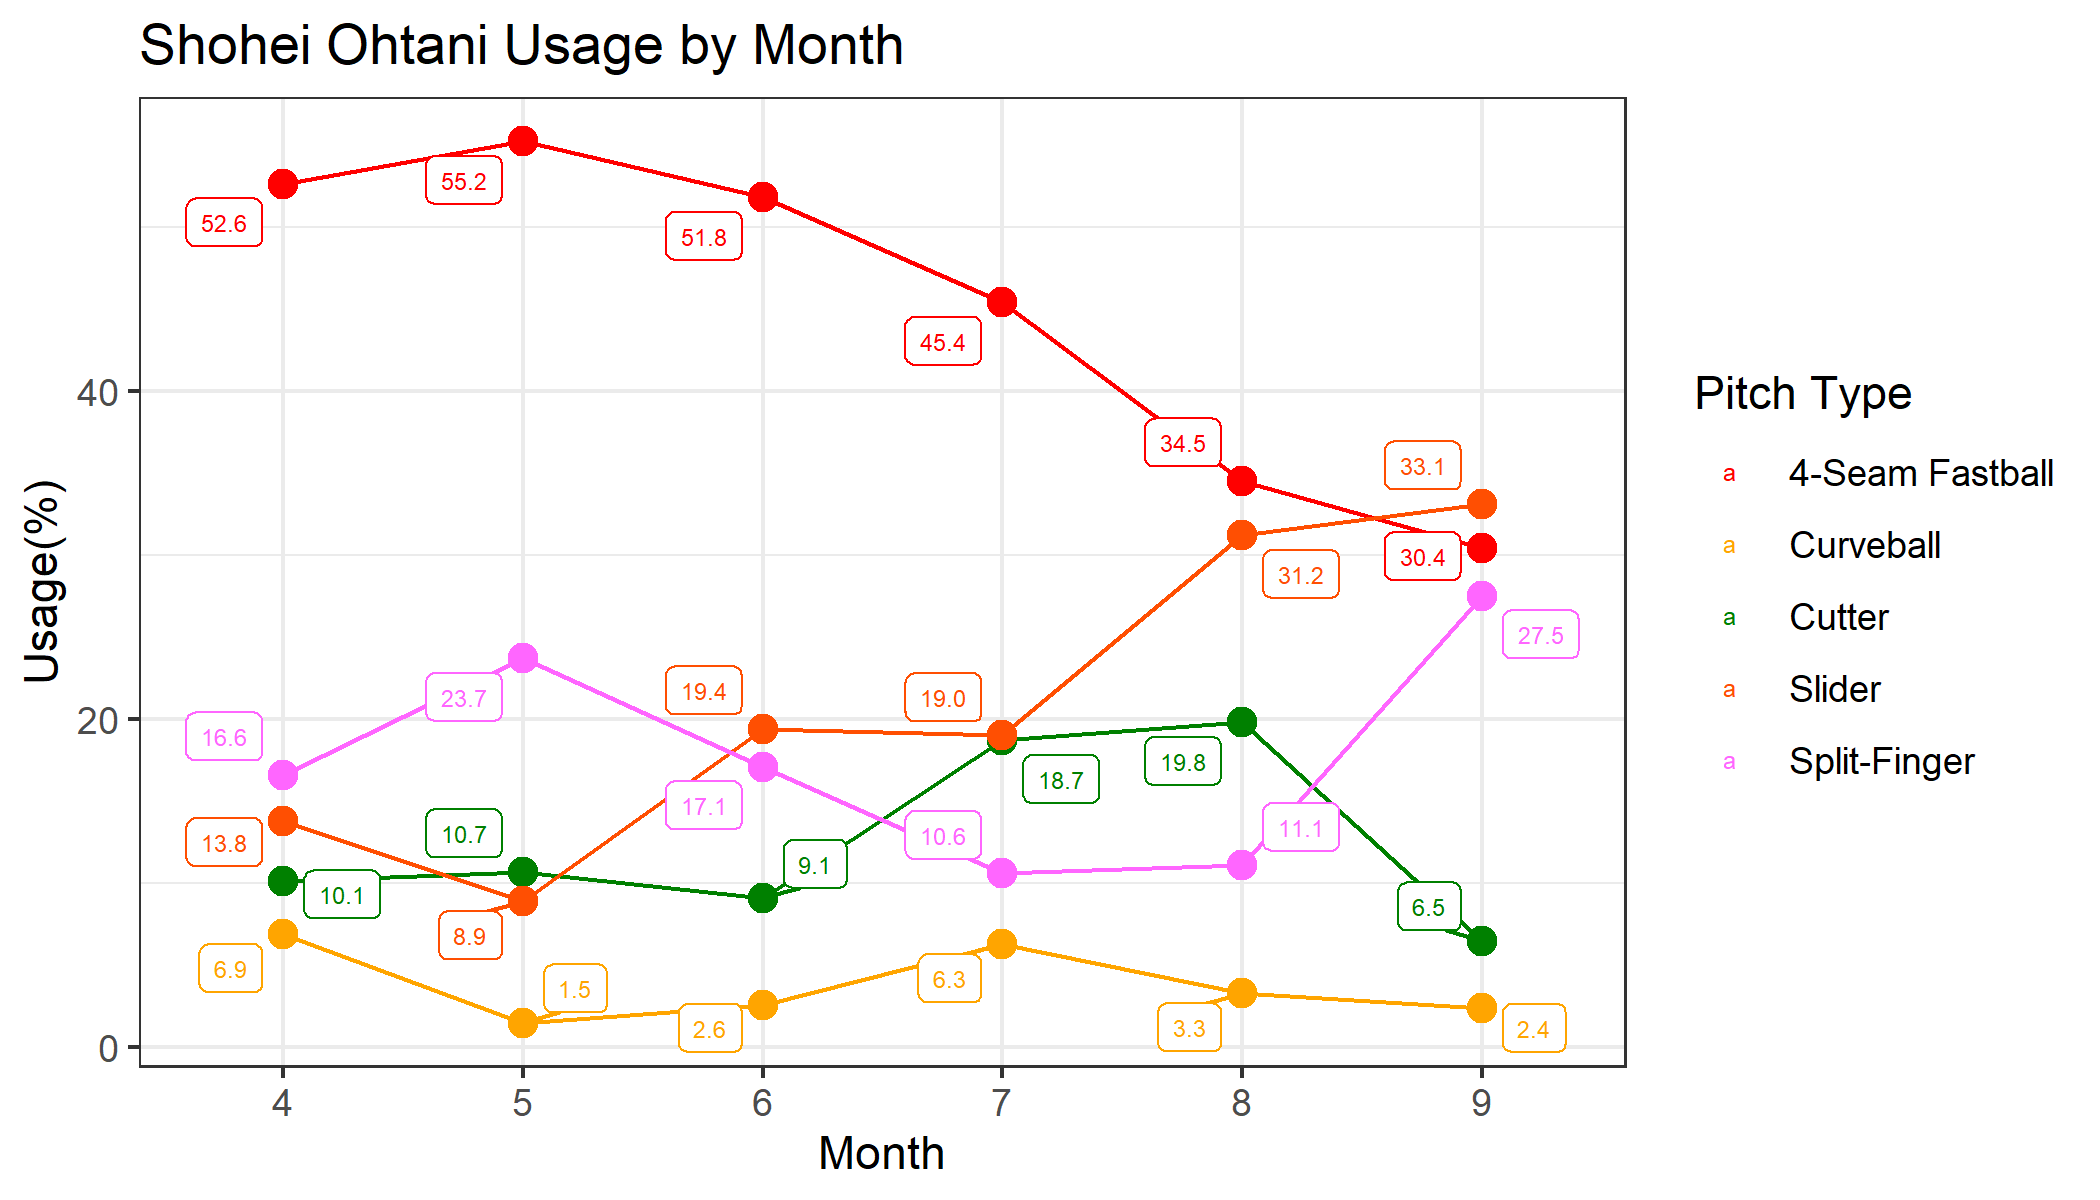
\includegraphics[width=0.65\linewidth]{figs/Ohtani_pitch_usage_byMonth} \end{center}
\end{block}
\end{frame}

\begin{frame}[fragile]{分析と結果の表示}
\protect\hypertarget{ux5206ux6790ux3068ux7d50ux679cux306eux8868ux793a}{}
\begin{itemize}
\tightlist
\item
  分析目的の設定
\item
  分析の一例:CollegeDistanceデータを用いた分析

  \begin{itemize}
  \tightlist
  \item
    操作変数法
  \end{itemize}
\item
  2群間の比較:\(t\)検定
\item
  最小二乗法
\item
  最尤法

  \begin{itemize}
  \tightlist
  \item
    ロジスティック回帰
  \end{itemize}
\end{itemize}

\begin{block}{計量分析を行う}
\protect\hypertarget{ux8a08ux91cfux5206ux6790ux3092ux884cux3046}{}
\begin{itemize}
\tightlist
\item
  データの要約・可視化が終わったら、因果関係を識別するための分析に取り組む
\item
  最も一般的なのは回帰分析
\end{itemize}

\[y_{i} = \alpha + \beta X_i + u_i\]

\begin{itemize}
\tightlist
\item
  説明変数の係数を推定し、説明変数の限界的な変化が被説明変数に対してどれだけ影響するかを推定したい
\item
  ここでは、Rで利用できるパッケージを使って分析の一例を示す
\end{itemize}
\end{block}

\begin{block}{AERパッケージの導入}
\protect\hypertarget{aerux30d1ux30c3ux30b1ux30fcux30b8ux306eux5c0eux5165}{}
\begin{itemize}
\tightlist
\item
  ペンギンのデータは簡潔で便利だが、経済学の分析に使うのはちょっと厳しそう
\item
  経済学向けのサンプルデータがあればいい
\item
  あります:AERパッケージ

  \begin{itemize}
  \tightlist
  \item
    \href{https://cran.r-project.org/web/packages/AER/AER.pdf}{CRAN}
  \item
    パッケージをライブラリで起動後、利用したいデータセットを\texttt{data()}関数で起動、データフレームが自動で取り込まれる
  \end{itemize}
\end{itemize}

\begin{Shaded}
\begin{Highlighting}[]
\FunctionTok{install.packages}\NormalTok{(}\StringTok{"AER"}\NormalTok{)}
\FunctionTok{library}\NormalTok{(AER)}
\FunctionTok{data}\NormalTok{(}\StringTok{"DataSetName"}\NormalTok{) }\CommentTok{\#好きなデータセットの名前、一覧はpdfを参照}
\end{Highlighting}
\end{Shaded}
\end{block}

\begin{block}{AERパッケージの利用}
\protect\hypertarget{aerux30d1ux30c3ux30b1ux30fcux30b8ux306eux5229ux7528}{}
\begin{Shaded}
\begin{Highlighting}[]
\FunctionTok{data}\NormalTok{(}\StringTok{"CollegeDistance"}\NormalTok{)}
\FunctionTok{print}\NormalTok{(}\FunctionTok{head}\NormalTok{(CollegeDistance))}
\end{Highlighting}
\end{Shaded}

\begin{verbatim}
##   gender ethnicity score fcollege mcollege home urban unemp wage distance
## 1   male     other 39.15      yes       no  yes   yes   6.2 8.09      0.2
## 2 female     other 48.87       no       no  yes   yes   6.2 8.09      0.2
## 3   male     other 48.74       no       no  yes   yes   6.2 8.09      0.2
## 4   male      afam 40.40       no       no  yes   yes   6.2 8.09      0.2
## 5 female     other 40.48       no       no   no   yes   5.6 8.09      0.4
## 6   male     other 54.71       no       no  yes   yes   5.6 8.09      0.4
##   tuition education income region
## 1 0.88915        12   high  other
## 2 0.88915        12    low  other
## 3 0.88915        12    low  other
## 4 0.88915        12    low  other
## 5 0.88915        13    low  other
## 6 0.88915        12    low  other
\end{verbatim}
\end{block}

\begin{block}{課題(佐々木ゼミ向け)}
\protect\hypertarget{ux8ab2ux984cux4f50ux3005ux6728ux30bcux30dfux5411ux3051}{}
\begin{itemize}
\tightlist
\item
  AERパッケージから好きなデータセットを使い

  \begin{itemize}
  \tightlist
  \item
    分析課題の設定:各データセットに元論文があるので、その研究テーマを使ってもOK
  \item
    データセットの要約:要約統計量、必要ならグループごとに分けたものを作成し、まとめておく
  \item
    なんでもいいので新しい変数を作ってみる
  \item
    データの可視化:分析課題を検証するにあたって必要そうな可視化を行う
  \item
    CollegeDistanceは解説で使うのでそれ以外で
  \end{itemize}
\item
  これを踏まえて、来週回帰分析などの分析手法を紹介します
\end{itemize}
\end{block}
\end{frame}

\begin{frame}{RMarkdownを用いたレポートの作成}
\protect\hypertarget{rmarkdownux3092ux7528ux3044ux305fux30ecux30ddux30fcux30c8ux306eux4f5cux6210}{}
\begin{itemize}
\tightlist
\item
  Markdown形式のドキュメント

  \begin{itemize}
  \tightlist
  \item
    数式フォントの利用
  \end{itemize}
\item
  コードブロックの作成
\item
  htmlドキュメントの作成
\item
  Wordファイルへの変換
\item
  Powerpointファイルへの変換
\item
  R Markdownを併用して論文作成・スライド作成の手間を省く
\end{itemize}

\begin{block}{Markdownとは}
\protect\hypertarget{markdownux3068ux306f}{}
\begin{itemize}
\tightlist
\item
  主にhtml(ウェブサイトなどで利用される形式)を手軽に出力するために考案された言語
\item
  Rの結果出力などに特化した形式:R Markdown

  \begin{itemize}
  \tightlist
  \item
    ここではR Markdownについて扱う
  \item
    htmlだけでなく、WordやPowerPointなど、使い慣れた形式にも変換可能
  \end{itemize}
\item
  分析結果をいちいちスクリーンショットしたり、体裁を整えるために出力をやり直したりする必要がなくなる

  \begin{itemize}
  \tightlist
  \item
    全てをR
    Markdownで完結させる必要はないので、例えば図や分析結果の出力をするためのWordファイルを作り、できたものをコピペするなどして使えば微調整も容易
  \end{itemize}
\end{itemize}
\end{block}
\end{frame}

\begin{frame}{おまけ:バージョン管理}
\protect\hypertarget{ux304aux307eux3051ux30d0ux30fcux30b8ux30e7ux30f3ux7ba1ux7406}{}
\begin{itemize}
\tightlist
\item
  論文執筆・輪読の資料報告は班単位で行うので、スライドや分析結果を複数人で作成・共有する必要がある
\item
  Dropbox, Github, Google Drive
  などでファイルごと共有しておくと、スライドをくっつけたり各自が修正したものをすり合わせる作業が削減できる、たぶん
\item
  覚えておいて損はないのでまあ興味があれば
\end{itemize}
\end{frame}

\end{document}
